\documentclass[12pt,letterpaper]{article}

\usepackage[T1]{fontenc}
\usepackage[utf8]{inputenc}
\usepackage{lmodern}
\usepackage{microtype}
\usepackage{amsmath,amssymb,mathtools}
\usepackage{booktabs}
\usepackage{array}
\usepackage[margin=1in]{geometry}
\usepackage{graphicx}
\graphicspath{{./}{figures/}{figures/global_all_v2/}}
\usepackage{setspace}
\usepackage[round,authoryear]{natbib}
\usepackage[hidelinks]{hyperref}
\usepackage{url}
\urlstyle{same}

\bibliographystyle{plainnat}

% Table note environment (finance-journal style: notes below the table)
\newcommand{\tabnote}[1]{\begin{minipage}{\linewidth}\vspace{4pt}\footnotesize\singlespacing #1\end{minipage}}

\newcommand{\PathQualityRows}{%
History-aware DLPM & 0.0485 & 0.3368 & 0.704 & 0.882 & 0.0075 \\
Contract-only DLPM & 0.0548 & 0.3626 & 0.735 & 0.767 & 0.0091 \\
Gaussian DDPM, simple loss & 0.0831 & 0.5461 & 0.226 & 0.154 & 0.0124 \\
Gaussian DDPM, finance-aware & 0.1521 & 0.9153 & 0.234 & 0.762 & 0.0100 \\
Historical block bootstrap & 0.0486 & 0.3297 & 0.864 & 1.139 & 0.0066 \\
Historical-drift GBM & 0.0498 & 0.3397 & 0.897 & 1.246 & 0.0102 \\
Conditional neural SDE & 0.0579 & 0.3774 & 0.794 & 1.537 & 0.0105 \\
Chronos-T5 zero-shot & 0.0542 & 0.3668 & 0.766 & 1.060 & 0.0093 \\
}
\newcommand{\EffectiveTailRows}{%
Realized & 2.71 / 2.20 & 2.93 / 2.92 & 9.75 & 2.93 / 3.33 & 1.01 / 1.01 \\
History-aware DLPM & 2.37 / 2.40 & 2.35 / 2.26 & 14.95 & 2.91 / 2.61 & 0.62 / 0.65 \\
Gaussian DDPM & 2.61 / 3.53 & 1.45 / 5.23 & 39.36 & 2.99 / 8.03 & 0.01 / 0.00 \\
Historical block bootstrap & 2.02 / 2.80 & 2.74 / 3.76 & 10.95 & 4.42 / 3.46 & 1.75 / 0.64 \\
Historical-drift GBM & 4.28 / 4.26 & 6.77 / 6.74 & 0.33 & 1.84 / 1.84 & 0.63 / 0.25 \\
}
\newcommand{\MainPnlRows}{%
Vanilla call & 0.91\% & 30.95\% & 61.27\% & 63.35\% & 0.86\% & 36.65\% & 0.06\% \\
Asian call & 0.36\% & 13.69\% & 59.74\% & 78.16\% & 0.33\% & 21.84\% & 0.03\% \\
Floating-strike lookback call & 0.28\% & 35.04\% & 55.96\% & 33.88\% & 0.61\% & 66.12\% & -0.33\% \\
}
\newcommand{\HedgedRows}{%
Vanilla call & 30.95\% & 0.91\% & 0.33\% & 60.84\% \\
Asian call & 13.69\% & 0.36\% & -0.04\% & 49.57\% \\
}
\newcommand{\SpreadRows}{%
Vanilla & 0.91\% & 30.95\% & 0.83\% & 27.49\% & 0.66\% & 21.61\% \\
Asian & 0.36\% & 13.69\% & 0.33\% & 12.00\% & 0.25\% & 9.06\% \\
Floating-strike lookback & 0.28\% & 35.04\% & 0.21\% & 29.94\% & 0.17\% & 20.97\% \\
}
\newcommand{\StructuredRows}{%
Accumulator & 11.01\% & 9.80\% & 9.33\% & 1.21pp & 45.82\% / 43.50\% / 52.71\% & -- \\
Snowball & 2.45\% & 1.86\% & 1.94\% & 0.59pp & 42.40\% / 39.09\% / 49.68\% & 99.96\% / 97.52\% / 98.49\% \\
}

\begin{document}
\pagenumbering{roman}

\begin{titlepage}
\begin{center}
\vspace*{0.35cm}
{\Large\bfseries Conditional Deep L\'evy Models for Exotic Derivatives:\\[5pt]
History-Aware Path Generation and P--Q Payoff Diagnostics\par}

\vspace{0.55cm}
{\large Helin Zhao\footnote{Johns Hopkins University.}
\qquad
Junchi Shen\footnote{University of Washington.}\par}

\vspace{0.15cm}
{\small Both authors contributed equally to this work.\par}

\vspace{0.25cm}
{Substantially revised arXiv and journal-submission version: July 2026\par}
\end{center}

\vspace{0.35cm}
\begin{abstract}
\noindent
We develop and audit a history-aware financial path generator based on
Denoising L\'evy Probabilistic Models (DLPMs) for conditional equity-index
path generation. The model combines symmetric
$\alpha$-stable diffusion noise with a conditional U-Net observing the
contract state, 60- and 252-day return histories, trend, drawdown, volatility
paths, country, and index identity. A chronological protocol evaluates a
frozen model on 6{,}824 untouched windows from eight Chinese and U.S. equity
indices. The final generator attains terminal CRPS 0.0485, path energy score
0.3368, a generated-to-realized volatility ratio of 0.882, and aggregate
signed terminal-median bias of $-0.46$ percentage points. It improves terminal
CRPS over contract-only DLPM and Gaussian diffusion controls, while an
unconditional historical block bootstrap remains competitive on pooled
marginal metrics. Against a stronger state-matched empirical control that
selects same-index, same-tenor training windows using pre-window volatility,
trend, and drawdown, DLPM lowers terminal CRPS from 0.0633 to 0.0485 (23.3\%);
for this state-matched CRPS comparison, joint calendar-block confidence
intervals remain below zero for block lengths
from 20 to 150 days.

We then use the learned physical-measure distribution in a transparent P--Q
payoff diagnostic. The Q side is an independently fitted Student-$t$
GARCH(1,1) benchmark with capped, unit-variance innovations and a numerical
log-mgf correction that enforces the stated discrete martingale restriction.
At the pre-specified $g=0.05$ dealer-spread setting and a $1\%S_0$ materiality
threshold, the aligned, unconditional P--Q diagnostic is 0.91\% of initial
spot for vanilla calls and 0.36\% for Asian calls. Complementary drift-neutral
and initial-delta diagnostics decompose this payoff difference into
direction-sensitive and residual components. Physical direction is an
important component of the raw gap; under the one-time RN-Q Delta diagnostic,
the Vanilla residual is 0.33\% of spot while the Asian residual is close to
zero. The P--Q framework is a belief-based payoff diagnostic, distinct from
an option-surface-calibrated pricing engine.
\end{abstract}

\enlargethispage{4\baselineskip}
\medskip
\noindent\textbf{Keywords:} denoising L\'evy probabilistic model; conditional diffusion;
exotic options; physical measure; risk-neutral benchmark; GARCH; scenario
generation; structured products.

\medskip
\noindent\textbf{JEL classification:} C45, C53, G12, G13, G17.
\end{titlepage}

\clearpage
\pagenumbering{arabic}
\doublespacing

\section{Introduction}\label{sec:introduction}
Financial institutions routinely value claims whose cash flows depend not
only on the terminal asset price but also on averages, extrema, observation
schedules, and the order in which market states are visited. Asian and
lookback options are canonical examples; accumulators and autocallable notes
combine path dependence with leverage, early termination, and nonlinear
coupon rules. Their risk cannot be summarized by a point forecast. What
matters is a conditional distribution over entire future paths.

Classical Monte Carlo valuation begins by specifying a stochastic process and
then averaging discounted payoffs. This workflow is transparent, but its
output inherits the restrictions of the assumed process. Geometric Brownian
motion imposes constant volatility and Gaussian increments. Local and
stochastic-volatility models are more flexible, yet they remain parsimonious
parametric representations of a market in which heavy tails, volatility
clustering, drawdowns, trend reversals, and regime-dependent dependence are
empirically prominent \citep{cont2001empirical}. These restrictions are
especially consequential for nonlinear claims: two models can agree on
one-step volatility and still disagree sharply on an Asian average, a running
maximum, or the sequence of states that activates a structured payoff.

Generative models offer a complementary route. Rather than committing to a
small set of diffusion coefficients, one can learn a conditional law of future
returns directly from historical paths. Denoising diffusion models are
attractive because they provide stable likelihood-inspired training, broad
support, and a natural mechanism for conditional scenario generation
\citep{ho2020ddpm,rasul2021timegrad}. A Gaussian forward process, however,
still builds light-tailed noise into the generative mechanism. For financial
returns, this is not an innocuous computational choice. Large moves are rare
but economically decisive, and the reverse process must represent them without
either suppressing tail mass or producing numerically uncontrolled paths.

This paper develops a heavy-tailed alternative based on the Denoising L\'evy
Probabilistic Model of \citet{shariatian2024dlpm}. The DLPM replaces Gaussian noise
with symmetric $\alpha$-stable innovations while retaining a tractable
variance-mixture representation. We combine this mechanism with a
history-aware conditional network and a finance-aware auxiliary objective.
The conditioning information is deliberately richer than the contract state:
it includes 60- and 252-day return sequences, rolling volatility, trend,
drawdown, downside risk, reversal indicators, country, and underlying index.
The resulting model is a conditional physical-measure path generator. It asks:
given what was observable at the start of a contract window, what distribution
of future index paths is plausible?

The second contribution is economic. A path generator should not be judged
only by a pooled return histogram. Small distributional differences can matter
greatly for nonlinear payoffs, while visually different paths can imply nearly
identical vanilla values. We therefore embed the frozen DLPM in a P--Q quoting
experiment. The P side represents the learned real-world belief. The Q side is
an independently fitted Student-$t$ GARCH(1,1) benchmark whose drift is
martingale-corrected under the simulated innovation law. The two models value
the same payoff; a trade is opened only when their valuation gap clears both
the dealer spread and a pre-specified execution threshold; the held-out
realized path determines ex-post P\&L. This construction converts path
differences into payoff-sensitive evidence without using downstream profits to
train or select the generator.

The distinction between P and Q is central. Historical conditional generation
and arbitrage-free pricing are related but different tasks. The DLPM is not
trained on option prices and is not subjected to a stochastic discount factor;
it therefore represents a physical-measure belief rather than a market-implied
risk-neutral law. Conversely, fitting a GARCH model to historical returns does
not by itself create a Q measure. Our benchmark explicitly sets the conditional
drift through a numerical log-mgf adjustment and verifies the discounted
martingale property. It remains a transparent benchmark Q, not a reconstruction
of the unique market-implied measure.

The empirical design is unusually broad for a financial diffusion study. The
sample contains CSI 300, CSI 500, CSI 1000, SSE Composite, S\&P 500, NASDAQ,
Dow Jones, and Russell 2000. The final protocol uses 59{,}240 training windows,
3{,}084 chronological validation windows, and 6{,}824 untouched test windows.
The validation period selects among EMA checkpoints; the test period is used
once for the final path and economic audit. Because the sliding windows overlap
and the indices share calendar shocks, we do not treat 6{,}824 windows as
independent observations. Economic uncertainty is estimated with joint
calendar-block bootstrap resampling at four block lengths.

The final results establish a broad conditional-generation capability. The
aggregate signed terminal-mean drift error is $-0.27$ percentage points and the
generated-to-realized volatility ratio is 0.882. Conditional fans anchor at
the observed index level, change scale across markets, and respond to the
pre-window state. Crucially, it lowers terminal CRPS by 23.3\% against a
same-index, same-tenor state-matched empirical control, with dependence-robust
confidence intervals excluding zero across all reported block lengths. The
aligned P--Q audit then converts these path differences into
payoff-sensitive diagnostics, with unconditional values of 0.91\% for vanilla
and 0.36\% for Asian calls at the primary dealer-spread setting and the
pre-specified $1\%S_0$ materiality threshold.

The paper makes five contributions:
\begin{enumerate}
\item It provides a full theoretical and computational formulation of
conditional Gaussian diffusion, finance-aware diffusion objectives, and
heavy-tailed DLPM training and sampling for financial paths.
\item It introduces a history-aware condition representation that combines
raw pre-start return sequences with interpretable trend, volatility,
drawdown, reversal, country, and index features.
\item It evaluates one global generator on eight equity indices under a
chronological train--validation--test protocol with target-end purging and no
payoff-based checkpoint selection.
\item It constructs and audits a martingale-corrected Student-$t$ GARCH RN-Q
benchmark, including post-truncation unit-variance normalization.
\item It links distributional path diagnostics to a payoff-sensitive P--Q
experiment with normalized results, spread sensitivity, and joint
calendar-block bootstrap uncertainty.
\end{enumerate}

Figure~\ref{fig:workflow} summarizes the complete system. The upper branch
learns the P-side conditional distribution; the lower branch constructs the
independent RN-Q benchmark; the final branch evaluates payoff beliefs against
held-out realizations.

\begin{figure}[ht]
\centering
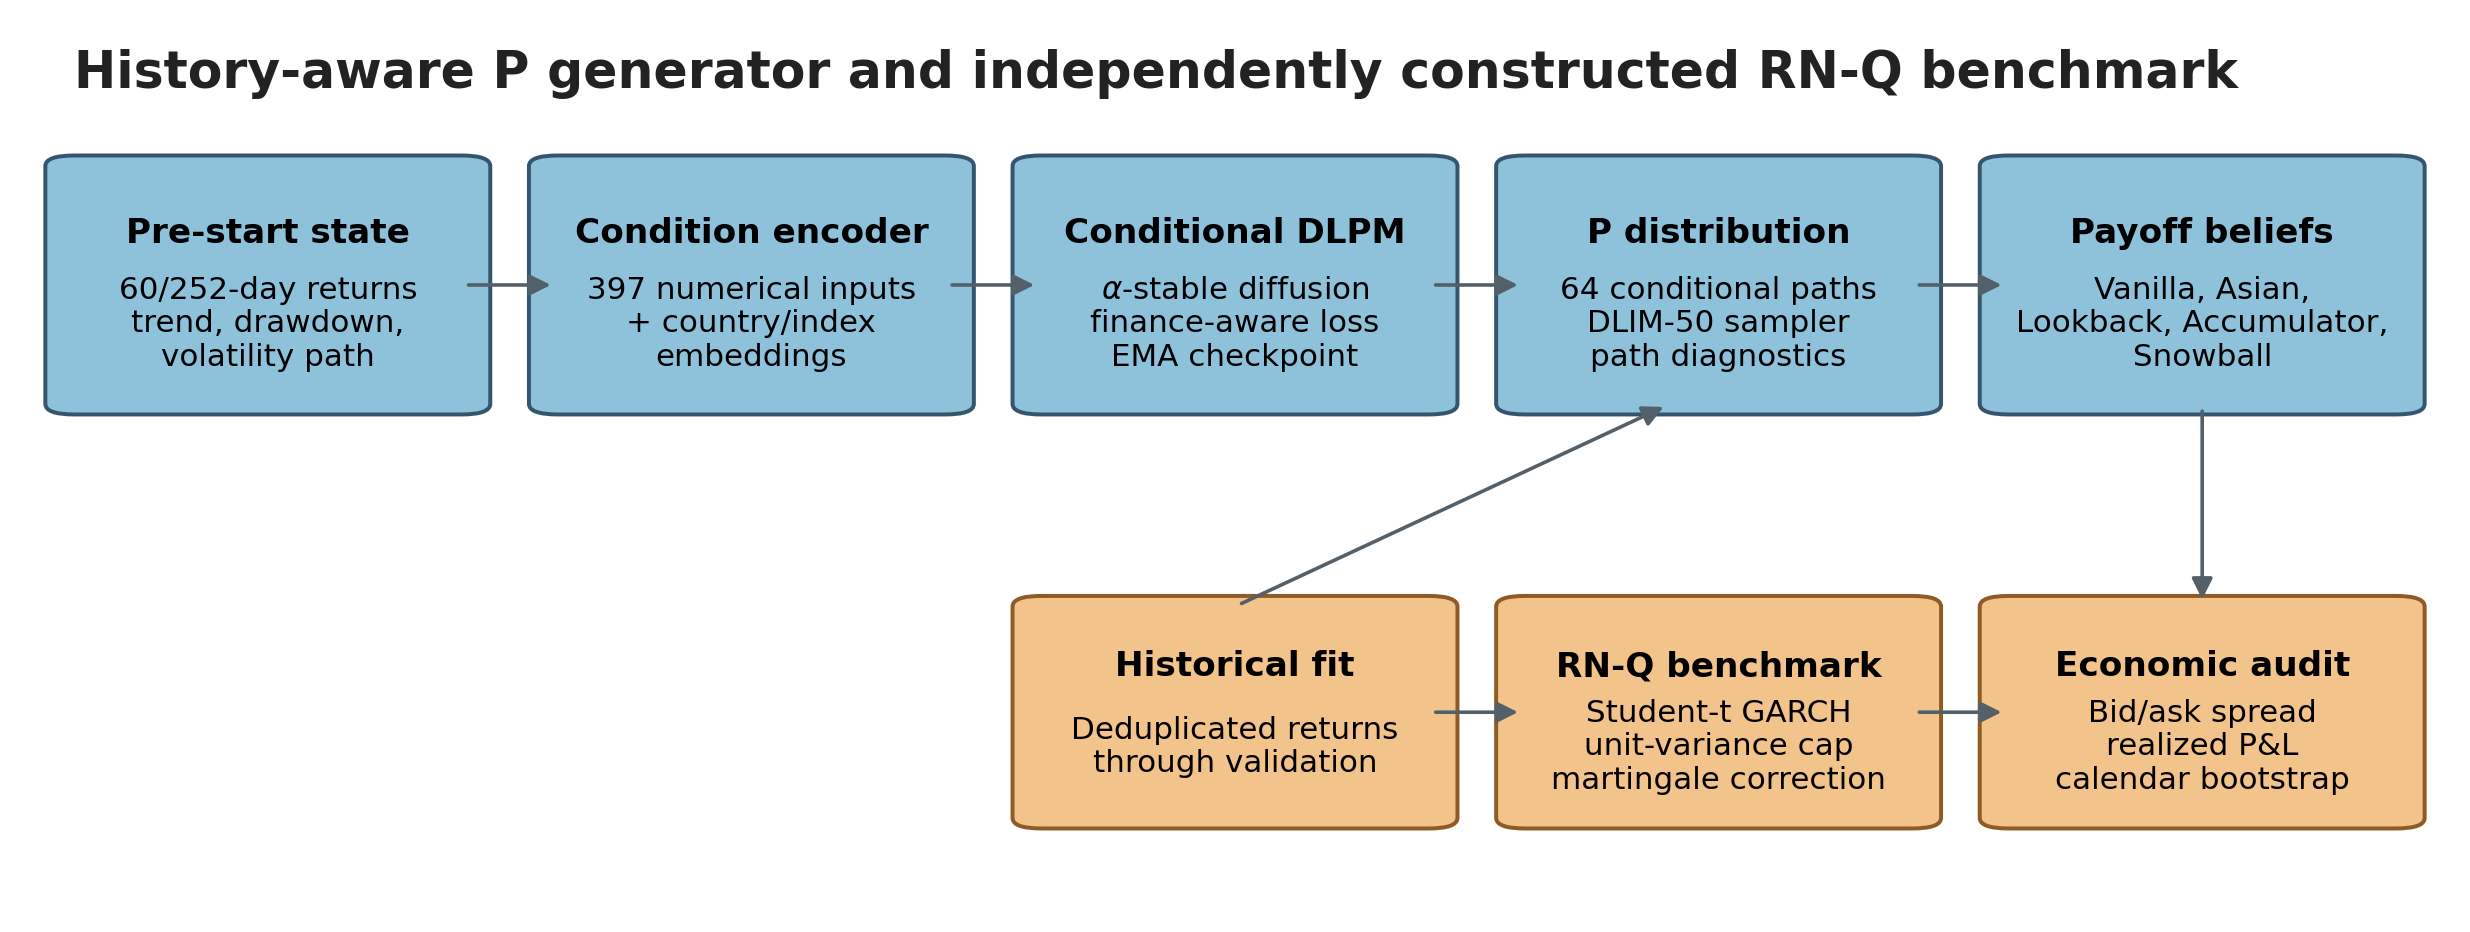
\includegraphics[width=\linewidth]{figures/final/01_system_workflow.png}
\caption{End-to-end research design. The DLPM learns conditional
physical-measure paths from pre-start information. The Student-$t$ GARCH
benchmark is fitted independently and martingale-corrected. Option payoffs and
the P--Q game are downstream audits and do not enter model training or
checkpoint selection.}
\label{fig:workflow}
\end{figure}

The remainder of the paper proceeds as follows.
Section~\ref{sec:literature} reviews exotic-option valuation, financial
generative models, and alternative time-series architectures.
Section~\ref{sec:data} presents the cross-market data and temporal protocol.
Section~\ref{sec:method} develops the Gaussian and L\'evy diffusion theory.
Section~\ref{sec:experiments} reports checkpoint selection and path quality.
Section~\ref{sec:game} constructs the RN-Q benchmark and presents the economic
results. Section~\ref{sec:limitations} consolidates the limitations and scope
of the study, and Section~\ref{sec:conclusion} concludes.

\section{Related Literature}\label{sec:literature}


\subsection{Pricing structured products and exotic options}

Industry practice relies on four methodologies \citep{deng2014valuation}:
simulation, which averages discounted payoffs over generated price paths and
suits strongly path-dependent products; numerical integration, when payoff
and density admit closed forms; decomposition into bonds, vanilla options,
and simpler exotics; and partial differential equation methods, which capture
continuous state dynamics at high solution cost. The Black--Scholes model,
despite its centrality for vanilla options, handles multi-layered structures
poorly given its risk-neutrality assumption and single volatility parameter.

A long literature refines these tools: Monte Carlo pricing from
\citet{boyle1977options}, jump-diffusion dynamics from
\citet{merton1976option}, Brownian-bridge quasi-Monte Carlo constructions
\citep{lin2008brownian}, ant colony optimization \citep{kumar2009aco}, and
tensor-network acceleration of lattice pricing \citep{vandamme2025tensor}.
Machine-learning approaches include LSTM option pricing
\citep{pimentel2025lstm}, generative adversarial models for arbitrage-free
implied volatility surfaces \citep{vuletic2025volgan}, and risk-neutral
pricing via GANs \citep{choi2025riskneutral}.

\subsection{Diffusion models for time series}

Denoising diffusion probabilistic models were established by
\citet{ho2020ddpm}, refined by the cosine schedule of
\citet{nichol2021improved}, and accelerated by the deterministic DDIM sampler
of \citet{song2020ddim}. TimeGrad \citep{rasul2021timegrad} pioneered
conditional diffusion for probabilistic time-series forecasting;
DiffSTOCK \citep{daiya2024diffstock} applies relational diffusion to equity
prediction; \citet{meijer2024rise} survey the area.

Diffusion models have recently become the leading generative approach for
financial time series. \citet{takahashi2025diffusion} show that denoising
diffusion models reproduce the stylized facts of asset
returns---heavy tails, volatility clustering, and dependence
structure---more faithfully than GANs and variational autoencoders, without
mode collapse; subsequent work extends the framework to conditional
multivariate generation with asset-specific and systematic covariates. Yet
the same literature emphasizes an open problem: no generator has fully
captured all stylized facts simultaneously, with tail behavior proving the
most stubborn. This gap motivates our heavy-tailed model class.

Classical diffusion is Gaussian-driven. For heavy-tailed data,
\citet{shariatian2024dlpm} propose Denoising L\'evy Probabilistic Models
(DLPMs), whose original formulation
replaces Gaussian increments with isotropic $\alpha$-stable noise,
$\alpha \in (1,2]$ \citep{samorodnitsky1994stable}. We retain the original
acronym and use ``conditional deep L\'evy model'' only as a descriptive label
for our financial adaptation, not as a renaming of the cited method. Our financial-path
implementation preserves the same stable-law mechanism but uses
\emph{coordinate-wise} stable scale mixing across ordered return coordinates,
instead of one path-level isotropic scale draw. Exploiting the variance-mixing
representation of stable laws, this retains DDPM's computational structure
with minimal changes while improving tail coverage; $\alpha = 2$ recovers the
Gaussian DDPM exactly. Given the well-documented heavy tails of asset returns
\citep{cont2001empirical}, DLPM is a natural generator for financial paths;
to our knowledge this paper is the first to evaluate it in a
derivatives-valuation setting.

\subsection{Alternative model families}

Financial market generators provide a closely related line of work.
\citet{wiese2020quantgans} use temporal-convolutional GANs to reproduce
long-range dependence and volatility clustering, while
\citet{kondratyev2019market} develop a restricted-Boltzmann-machine market
generator for dependence-aware scenario sampling. Signature methods replace a
learned discriminator with path-signature distances:
\citet{liao2024sigwasserstein} learn conditional time-series laws through a
Sig-Wasserstein objective. For derivative applications,
\citet{cuchiero2020ganlsv} calibrate neural local-stochastic-volatility models
to option prices, and \citet{buehler2019deephedging} learn hedging policies
under frictions. These studies establish complementary benchmarks for
scenario fidelity, risk-neutral calibration, and downstream hedging. Our
setting differs by learning a physical-measure, history-conditioned path law
with an explicit heavy-tailed diffusion mechanism and then auditing its
payoff implications against an independently constructed RN-Q benchmark.

Two further families compete in this space. \emph{Neural stochastic
differential equations} parameterize the drift and diffusion of an SDE by
neural networks, trained by likelihood or adversarial criteria
\citep{gierjatowicz2020neural}; imposing no-arbitrage constraints yields
market models suitable for risk-neutral applications
\citep{cohen2023neuralsde}. \emph{Time-series foundation models} such as
Chronos \citep{ansari2024chronos} and TimesFM \citep{das2024timesfm} are
transformers pretrained on billions of observations that produce zero-shot
probabilistic forecasts; however, generic foundation models tend to
underperform domain-specific architectures on financial data, and their
uncertainty calibration remains an open concern. Because both families are
natural alternatives to diffusion generators, our empirical study includes a
conditional neural-SDE baseline trained on identical data
(Section~\ref{sec:experiments}), positioning the diffusion results against the
classical SDE paradigm rather than against Gaussian Monte Carlo alone.

\section{Data and Experimental Protocol}\label{sec:data}

\subsection{Markets, dates, and window construction}

The data set covers eight broad equity indices in two large markets:
\begin{center}
CSI~300, CSI~500, CSI~1000, SSE Composite, S\&P~500, NASDAQ, Dow Jones, and
Russell~2000.
\end{center}
The raw collection spans 1 January 2014 through 1 August 2025. Chinese index
levels are obtained from AKShare (tickers 000300, 000905, 000852, and 000001),
and U.S. adjusted index series from Yahoo Finance (\texttt{\^GSPC},
\texttt{\^IXIC}, \texttt{\^DJI}, and \texttt{\^RUT}). The series are price-index
or provider-adjusted index levels, not total-return indices. Chinese rates use
SHIBOR 1-, 3-, 6-, and 12-month tenors; U.S. rates use FRED DGS1MO, DGS3MO,
DGS6MO, and DGS1. Rates are matched to contract tenor, converted to annual
decimals, and forward-filled on the local business-day calendar.

A 252-trading-day
pre-start history requirement and complete-target filtering determine the
usable range. Windows have calendar maturities of 30, 90, 180, and 365
days and record initial price, realized future path, historical volatility,
risk-free rate, country, and index identity.

\begin{table}[ht]
\singlespacing
\centering
\caption{Chronological sample construction}
\label{tab:datasplit}
\begin{tabular}{lrrrr}
\toprule
Split & Windows & Earliest start & Latest start & Latest target end \\
\midrule
Training & 59{,}240 & 2015-01-02 & 2022-11-11 & 2022-12-13 \\
Validation & 3{,}084 & 2023-01-03 & 2023-10-02 & 2023-11-01 \\
Test & 6{,}824 & 2024-01-02 & 2025-06-06 & 2025-07-06 \\
\bottomrule
\end{tabular}
\tabnote{Counts are after target-end purging. Target end is reconstructed from
the window start, contractual calendar horizon, and stored realized path, and
was checked against the realized-price archive. The test set contains 827
windows for each Chinese index and 879 for each U.S. index.}
\end{table}

The split is chronological and materialized before training. For each
underlying, a target end date is reconstructed from its ordered trading
calendar and stored path length. A window in the training or validation split
is retained only if its estimated target end precedes the next split boundary
by at least 20 calendar days. The implementation labels this operation as a
purge/embargo; the actual code uses a 20-calendar-day buffer rather than
claiming 20 exchange-specific trading days. This distinction is documented
because it matters for exact replication. The resulting maximum target dates
in Table~\ref{tab:datasplit} leave visible separation from the following
split's start.

\subsection{Returns, scales, and historical state}

For index level $S_t$, daily log return is
\begin{equation}
r_t=\log(S_t/S_{t-1}),
\end{equation}
and annualized historical volatility over $n$ observations is
\begin{equation}
\sigma_{\mathrm{ann}}
=\sqrt{252}\left(\frac{1}{n-1}\sum_{t=1}^{n}(r_t-\bar r)^2\right)^{1/2}.
\end{equation}
The model represents the target in scaled log-return space,
\begin{equation}
x_{0,t}=r_t/s_{\mathrm{vol}}, \qquad s_{\mathrm{vol}}=0.09,
\end{equation}
and reconstructs levels by exact anchoring at $S_0$:
\begin{equation}
\widehat S_t=S_0\exp\left(s_{\mathrm{vol}}\sum_{j=1}^{t}\widehat x_{0,j}\right).
\label{eq:reconstruct}
\end{equation}
Equation~\eqref{eq:reconstruct} guarantees that every generated path starts at
the observed contract level. Variable-tenor windows are padded to length 252
and accompanied by a validity mask; padded entries do not contribute to the
training objective. Price observations with missing dates or levels are
dropped rather than interpolated. Exchange holidays and suspensions therefore
shorten the stored realized path; payoff evaluation uses the recorded
\texttt{actual\_trading\_days} and never fabricates unavailable prices.

The numerical condition contains 397 entries. It combines contemporaneous
contract variables with strictly pre-start information: raw 60- and 252-day
return sequences, a 60-day volatility path, 20/60/252-day trends, current and
maximum drawdown, realized and downside volatility, recent reversal,
momentum acceleration, and ratios between short- and long-horizon volatility.
Two categorical identifiers encode country and underlying. Learned embeddings
allow the global model to share common financial structure while retaining
market-specific behavior.

The raw sequences and summary variables play different roles. Sequences
retain local temporal ordering; summaries expose low-frequency state variables
that a convolutional encoder might otherwise learn inefficiently. This
combination is particularly useful at long horizons, where a network must
distinguish a high-volatility rebound from a low-volatility trend even when
their one-day return distributions overlap.

\subsection{Dependence and effective sample size}

Sliding windows are intentionally dense because they expose the model to many
conditional states. They do not create an equal number of independent
experiments. Adjacent windows share both historical context and forward
targets, and indices within the same country share market-wide shocks.
Accordingly, the paper never interprets 6{,}824 as an effective independent
sample size. Path metrics are descriptive averages over the complete held-out
set. Economic uncertainty is estimated by sampling common calendar blocks for
all assets, preserving both serial overlap and cross-index synchronization.
We report 20- and 60-day blocks as the primary dependence-robust inference
checks, 90-, 120-, and 150-day blocks as medium-horizon sensitivities, and
180- and 252-day blocks as long-dependence sensitivities, each with 2{,}000
replications. The latter two have only three nonempty calendar blocks and are
reported for transparency rather than treated as decisive inference.

\subsection{Validation and information discipline}

The network is optimized for 16{,}000 steps. EMA checkpoints at 4{,}000,
8{,}000, 12{,}000, and 16{,}000 steps are evaluated on the validation period
with fixed random seeds and the deployed 50-step sampler. Selection uses the
pre-specified validation score
\begin{equation}
\mathcal S_{\rm val}=|\widehat C_{0.9}-0.9|+0.5\,\mathrm{CRPS}
+0.25\,\mathrm{Energy}+0.5|\log(\widehat\sigma/\sigma)|
+0.25|\Delta\mathrm{ACF}|+0.1|\Delta\mathrm{Median}|.
\end{equation}
The component diagnostics additionally include terminal quantiles, tail
behavior, autocorrelation, and drawdown. No option
payoff, P--Q profit, or test observation enters checkpoint selection.
EMA-12000 is frozen before the 2024--2025 test audit.

\section{Methodology}\label{sec:method}


\subsection{Gaussian conditional diffusion}\label{sec:ddpm}

The forward process of a DDPM is a Markov chain that gradually corrupts the
data $x_0 \in \mathbb{R}^{B \times C \times L}$ with Gaussian noise,
\begin{equation}
q(x_t \mid x_{t-1}) = \mathcal{N}\bigl(x_t;\ \sqrt{1-\beta_t}\,x_{t-1},\
\beta_t I\bigr),
\end{equation}
under the cosine schedule $\beta_t$ of \citet{nichol2021improved} with
$T = 1000$ steps in the final clean-split deployment. With $\alpha_t = 1 - \beta_t$ and
$\bar\alpha_t = \prod_{i \le t} \alpha_i$, the marginal admits the
reparameterization
\begin{equation}
x_t = \sqrt{\bar\alpha_t}\,x_0 + \sqrt{1-\bar\alpha_t}\,\epsilon_t,
\qquad \epsilon_t \sim \mathcal{N}(0, I).
\end{equation}

The reverse process approximates $q(x_{t-1} \mid x_t, x_0)$ by a Gaussian
transition conditioned on contract features $c$,
\begin{equation}
p_\theta(x_{t-1} \mid x_t, c) = \mathcal{N}\bigl(x_{t-1};\
\mu_\theta(x_t, t, c),\ \tilde\beta_t I\bigr),
\end{equation}
where the conditional U-Net (Appendix~\ref{app:architecture}) outputs
$\hat x_0 = f_\theta(x_t, t, c)$ and the posterior mean and variance follow
from Bayes' rule for the Gaussian chain:
\begin{equation}
\tilde\mu_t(x_t, \hat x_0)
= \frac{\sqrt{\bar\alpha_{t-1}}\,\beta_t}{1-\bar\alpha_t}\,\hat x_0
+ \frac{\sqrt{\alpha_t}\,(1-\bar\alpha_{t-1})}{1-\bar\alpha_t}\,x_t,
\qquad
\tilde\beta_t = \frac{1-\bar\alpha_{t-1}}{1-\bar\alpha_t}\,\beta_t .
\end{equation}

For fast generation we use the deterministic DDIM sampler
\citep{song2020ddim}: for a subsequence $\{\tau_i\} \subset \{1,\dots,T\}$,
\begin{equation}
x_{\tau_{i-1}}
= \sqrt{\bar\alpha_{\tau_{i-1}}}\,
\underbrace{\frac{x_{\tau_i} - \sqrt{1-\bar\alpha_{\tau_i}}\,
\hat\epsilon_{\tau_i}}{\sqrt{\bar\alpha_{\tau_i}}}}_{\hat x_0}
+ \sqrt{1-\bar\alpha_{\tau_{i-1}} - \sigma_{\tau_i}^2}\;\hat\epsilon_{\tau_i}
+ \sigma_{\tau_i}\, z,
\qquad z \sim \mathcal{N}(0, I),
\end{equation}
with $\sigma_{\tau_i} = 0$ in the fully deterministic case.

\subsection{Training objective I: simple loss}\label{sec:simpleloss}

The \emph{simple} objective is the standard masked denoising regression of
Eq.~\eqref{eq:simple} applied to the network's clean-sequence prediction:
\begin{equation}
\mathcal{L}_{\mathrm{simple}}
= \mathbb{E}_{t,\,x_0,\,\epsilon}
\Bigl[\bigl\| M \odot \bigl(f_\theta(x_t, t, c) - x_0\bigr) \bigr\|_2^2
\big/ \textstyle\sum M \Bigr].
\label{eq:simple}
\end{equation}
This is the direct analogue of the original DDPM objective and embeds no
financial domain knowledge.

\subsection{Training objective II: composite finance-aware loss}\label{sec:complexloss}

Financial returns exhibit stylized facts---volatility clustering, heavy
tails, skewness, and characteristic spectra---that pure mean-squared error
does not explicitly reward \citep{cont2001empirical}. The \emph{composite}
objective augments Eq.~\eqref{eq:simple} with auxiliary regularizers
computed between the predicted clean sequence $\hat x_0$ and the target
$x_0$, all masked as in Eq.~\eqref{eq:simple}:
\begin{align}
L_{\mathrm{jump}} &= \bigl\| (\hat x_{0,i+1} - \hat x_{0,i}) -
(x_{0,i+1} - x_{0,i}) \bigr\|_1
&& \text{(relative jumps)}, \\
L_{\mathrm{vol}} &= \mathrm{SmoothL1}\bigl(\mathrm{Std}(\hat
x_{0,\mathrm{win}}),\ \mathrm{Std}(x_{0,\mathrm{win}})\bigr)
&& \text{(volatility clustering)}, \\
L_{\mathrm{gvol}} &= \bigl|\sigma_{\mathrm{pred}} -
\sigma_{\mathrm{true}}\bigr|
&& \text{(global volatility)}, \\
L_{\mathrm{kurt}} &= \bigl(K_{\mathrm{pred}} - K_{\mathrm{true}}\bigr)^2,
\quad K = \mathbb{E}[z^4] - 3
&& \text{(heavy tails)}, \\
L_{\mathrm{skew}} &= \bigl(\mathbb{E}[z_{\mathrm{pred}}^3] -
\mathbb{E}[z_{\mathrm{true}}^3]\bigr)^2
&& \text{(skewness)}, \\
L_{\mathrm{drift}} &= \Bigl(\textstyle\sum_i \Delta\hat x_{0,i} -
\sum_i \Delta x_{0,i}\Bigr)^2
&& \text{(terminal drift)}, \\
L_{\mathrm{quant}} &= \textstyle\sum_{\tau \in \{0.01, 0.99\}}
L_\tau\bigl(q_\tau(x_0),\ q_\tau(\hat x_0)\bigr)
&& \text{(extreme quantiles)}, \\
L_{\mathrm{spec}} &= \mathrm{SmoothL1}\bigl(\hat P_{\mathrm{norm}},\
P_{\mathrm{norm}}\bigr)
&& \text{(power spectrum)},
\end{align}
where $z$ denotes the standardized sequence, $L_\tau$ is the pinball loss of
\citet{wang2019pinball} at quantile $\tau$, and
$P_{\mathrm{norm}}[k] = P[k]/\max_k P[k]$ is the normalized discrete Fourier
magnitude spectrum. The extreme-quantile pair $\tau \in \{0.01, 0.99\}$
penalizes underestimation of both tails asymmetrically, sharpening the
delineation of downside risk and upside potential.

Because the auxiliary terms live on heterogeneous scales, each is normalized
by an exponential moving average (EMA) of its own magnitude, and all
auxiliary weights are annealed linearly from zero over a warm-up phase
($s = \min(1, \mathrm{step}/\mathrm{warmup})$):
\begin{equation}
\mathcal{L}_{\mathrm{complex}}
= \mathcal{L}_{\mathrm{simple}}
+ s \sum_{k \in \mathcal{K}} \lambda_k\,
\frac{L_k}{\mathrm{EMA}[L_k] + \varepsilon},
\label{eq:complex}
\end{equation}
with base weights
$(\lambda_{\mathrm{jump}}, \lambda_{\mathrm{vol}}, \lambda_{\mathrm{gvol}},
\lambda_{\mathrm{kurt}}, \lambda_{\mathrm{skew}}, \lambda_{\mathrm{drift}},
\lambda_{\mathrm{quant}}, \lambda_{\mathrm{spec}})
= (0.5, 3.5, 8, 5, 0.5, 2, 3, 2)$.

\subsection{Heavy-tailed diffusion: the DLPM}\label{sec:dlpm}

Gaussian diffusion imposes light-tailed increments on the forward chain. The
original Denoising L\'evy Probabilistic Model of
\citet{shariatian2024dlpm} is isotropic. Our deployed
financial-path variant instead uses coordinate-wise symmetric $\alpha$-stable
innovations: for return coordinate $j$,
$\varepsilon^{(\alpha)}_{t,j}\sim\mathcal{S}\alpha\mathcal{S}(1)$,
independently across $j$, with stability index $\alpha\in(1,2]$.
This avoids a single path-level scale draw imposing common shocks across every
ordered return coordinate. The forward chain is applied coordinate-wise,
\begin{equation}
x_{t,j} = \gamma_t x_{t-1,j} + \sigma_t\varepsilon^{(\alpha)}_{t,j},
\qquad t = 1, \dots, T,
\end{equation}
or, equivalently in vector notation,
\begin{equation}
x_t = \gamma_t\, x_{t-1} + \sigma_t\, \varepsilon_t^{(\alpha)},
\qquad t = 1, \dots, T,
\end{equation}
under a \emph{scale-preserving} schedule: with
$\bar\gamma_t = \prod_{i\le t}\gamma_i$, the stability property gives the
marginal
\begin{equation}
x_t = \bar\gamma_t\, x_0 + \bar\sigma_t\, \bar\varepsilon^{(\alpha)},
\qquad
\bar\sigma_t = \bigl(1 - \bar\gamma_t^{\,\alpha}\bigr)^{1/\alpha},
\end{equation}
so $\bar\gamma_t^{\,\alpha} + \bar\sigma_t^{\,\alpha} = 1$ generalizes
variance preservation. We derive $\gamma_t = \alpha_t^{1/\alpha}$ from the
same cosine schedule as the Gaussian model, so both models traverse
comparable signal-to-noise trajectories.

Computations with stable laws become Gaussian conditionally on auxiliary
variables \citep{samorodnitsky1994stable}. In the deployed coordinate-wise
variant, each return coordinate admits the \emph{variance-mixing}
representation
\begin{equation}
\varepsilon^{(\alpha)}_{t,j} \overset{d}{=} \sqrt{a_{t,j}}\; Z_{t,j},
\qquad
a_{t,j} \sim \mathcal{S}_{\alpha/2}^{+},\quad Z_{t,j}\sim\mathcal{N}(0,1),
\label{eq:mixing}
\end{equation}
with $\mathcal{S}_{\alpha/2}^{+}$ the totally skewed positive
$(\alpha/2)$-stable law. The implementation uses the
Chambers--Mallows--Stuck convention equivalent to stability
$\gamma=\alpha/2$, skewness $\beta=1$, location zero, and scale
$c_A=2\cos(\pi\alpha/4)^{2/\alpha}$. For numerical stability the deployed
sampler replaces $a_{t,j}$ by $\min(a_{t,j},100)$. Consequently, the
implemented forward law is a capped stable-mixture approximation rather than
an unbounded exact $\alpha$-stable law; all reported model and sampler results
use this same convention. Conditionally on the coordinate-wise chain
$A=(a_{t,j})_{t,j}$, the forward process is Gaussian with stochastic diagonal
variances. The following posterior recursion applies element-wise, with
$\Sigma_{t,j}$ and $\Gamma_{t,j}$ replacing the scalar notation:
\begin{equation}
\Sigma_{t,j} = \sigma_t^2\, a_{t,j} + \gamma_t^2\, \Sigma_{t-1,j},
\quad
\Gamma_{t,j} = 1 - \frac{\gamma_t^2\,\Sigma_{t-1,j}}{\Sigma_{t,j}},
\quad
\tilde m_{t-1,j} = \frac{x_{t,j} - \bar\sigma_t\,\Gamma_{t,j}\,\varepsilon_{t,j}}{\gamma_t},
\quad
\tilde\Sigma_{t-1,j} = \Gamma_{t,j}\, \Sigma_{t-1,j}.
\label{eq:posterior}
\end{equation}

\paragraph{Training objective III: standard DLPM loss.}
The network predicts the chain noise
$\varepsilon_t = (x_t - \bar\gamma_t x_0)/\bar\sigma_t$. A training sample is
constructed via Eq.~\eqref{eq:mixing},
\begin{equation}
a_t \sim \mathcal{S}_{\alpha/2}^{+}, \quad z \sim \mathcal{N}(0, I), \quad
x_t = \bar\gamma_t\, x_0 + \bar\sigma_t \sqrt{a_t}\, z,
\qquad \varepsilon_t = \sqrt{a_t}\, z,
\end{equation}
and the \emph{standard loss} is the $L_p$ objective
\begin{equation}
\mathcal{L}_{\mathrm{DLPM}}
= \mathbb{E}_{t,\,x_0,\,a_t,\,z}
\Bigl[\bigl\| M \odot \bigl(\hat\varepsilon_\theta(x_t, t, c) -
\varepsilon_t\bigr)\bigr\|_p \Bigr].
\label{eq:dlpmloss}
\end{equation}
Because $\alpha$-stable noise has infinite variance for $\alpha < 2$, the
exponent must respect a moment constraint; we use the \emph{unsquared} $L_2$
norm---an order-one moment of
$\|\varepsilon\|_2 = \sqrt{a}\,\|Z\|_2$---which is finite for all
$\alpha > 1$. \citet{shariatian2024dlpm} additionally propose a
median-of-means estimator over multiple draws of $a_t$; the single-draw
estimator proved sufficient at our scale. For numerical stability, extreme
draws of $a_t$ are clamped at $a_{\max} = 100$. In the deployed configuration,
the coordinate-wise innovation supplied to the denoising chain is also
symmetrically clipped at $\lvert\varepsilon\rvert\leq 2$, matching the
$2\tanh(\cdot)$ output range of the U-Net. Thus the implemented process is a
numerically truncated heavy-tailed DLPM rather than an unbounded stable law;
the stable scale mixture remains the tail-generating mechanism within this
explicit computational support. The controlled standard-DLPM ablation does not use
the financial regularizers of Section~\ref{sec:complexloss}. The final
full-sample model used for the reported path and P--Q experiments is a
history-aware conditional DLPM that adds a small, clipped finance-aware
auxiliary term to Eq.~\eqref{eq:dlpmloss}. Its warm-up and scale are reported
in Appendix~\ref{app:hyper}; this separates the theoretical DLPM objective
from the engineering stabilization used in the final production run.

\paragraph{Sampling.}
\emph{Ancestral} sampling draws the auxiliary chain $A$ and initial noise
$x_T = \bar\sigma_T \varepsilon^{(\alpha)}$, then iterates the Gaussian
posterior of Eq.~\eqref{eq:posterior} with
$\varepsilon_t \to \hat\varepsilon_\theta(x_t, t, c)$. Because the variances
$\Sigma_t$ are driven by heavy-tailed $a_t$, individual reverse trajectories
can take occasional large steps---precisely the mechanism that reproduces
jumps. \emph{DLIM}, the deterministic skip-step analogue of DDIM, transports
the state exactly between noise levels of a subsequence $\{\tau_i\}$:
\begin{equation}
x_{\tau_{i-1}}
= \frac{\bar\gamma_{\tau_{i-1}}}{\bar\gamma_{\tau_i}}
\bigl(x_{\tau_i} - \bar\sigma_{\tau_i}\,\hat\varepsilon_{\tau_i}\bigr)
+ \bar\sigma_{\tau_{i-1}}\, \hat\varepsilon_{\tau_i}.
\label{eq:dlim}
\end{equation}

\section{Model Selection and Held-Out Path Evaluation}
\label{sec:experiments}

\subsection{What the comparison is designed to identify}

The final-split comparison holds the same chronological test set fixed across
contract-only DLPM, history-aware Gaussian DDPM with simple loss,
history-aware Gaussian DDPM with finance-aware loss, the frozen history-aware
DLPM, historical block bootstrap, historical-drift GBM, conditional neural
SDE, and Chronos-T5 zero-shot.
The neural families use repeated seeds where applicable. This design separates
the value of historical conditioning and the heavy-tailed diffusion mechanism
from the value of a generic physical-measure baseline; downstream payoff
results do not participate in model selection.

\subsection{Production training and checkpoint selection}

The final model uses $T=1000$ diffusion steps, stability index
$\alpha=1.9$, a U-Net base width of 64 with channel multipliers
$(1,2,4,8)$, and a 128-dimensional fused condition embedding. Training uses
Adam with learning rate $10^{-5}$, batch size 32, cosine decay, EMA decay
0.995, and regime-balanced sample weights capped at 1.5. The cap is applied
after normalization so that the realized maximum weight cannot exceed the
configured ceiling. The finance-aware term is warmed up for 1{,}000 steps,
scaled by 0.07, and clipped at 2.5 before being added to the DLPM denoising
objective; model-space returns and sampled $x_0$ are clipped at 1.25 and 1.35,
respectively. Appendix Table~\ref{tab:financeweights} reports every sub-weight.

Regime balancing is market-agnostic. Every training window receives a weight
from the same transformation of volatility, trend, and drawdown state; country
is used for stratification, not for a country-specific rule. The objective is
to prevent the large mass of quiet windows from overwhelming high-volatility
and reversal states while preserving the empirical market composition.

EMA-12000 achieves the best validation composite score among the pre-specified
production checkpoints. It is frozen before generation of the final test
archive. Selection uses path-distribution diagnostics only; no payoff result
or test-set comparison is used to choose the reported checkpoint.

\subsection{Full held-out path results}

Table~\ref{tab:pathquality} reports the final-split path audit. The frozen
EMA-12000 DLIM-50 model has terminal CRPS 0.0485 and path energy score 0.3368.
Its aggregate signed terminal-drift error is $-0.27$ percentage points and
its generated-to-realized volatility ratio is 0.882. As an auxiliary pooled
terminal-distribution diagnostic, it obtains KS statistic 0.1004,
Wasserstein distance 0.0228, and quantile--quantile $R^2$ of 0.8803. These
statistics summarize marginal terminal-shape agreement and complement, rather
than replace, the conditional ensemble scores and interval coverage in
Table~\ref{tab:pathquality}. These results accompany
material improvements over the contract-only and Gaussian controls, and are
consistent with contributions from both the history-aware architecture and
the heavy-tailed mechanism beyond a contract-only diffusion specification;
the fully budget- and loss-matched isolation of the mechanism is the
$\alpha=2$ ablation noted in Section~\ref{sec:limitations}. Detailed centre-dispersion
diagnostics are reported separately to guide future conditional calibration.

\begin{table}[ht]
\singlespacing
\centering
\caption{Final-split held-out path quality and representative controls}
\label{tab:pathquality}
\resizebox{\textwidth}{!}{%
\begin{tabular}{lrrrrr}
\toprule
Model & Terminal CRPS & Energy score & 90\% coverage & Volatility ratio & Tail error \\
\midrule
\PathQualityRows
\bottomrule
\end{tabular}
}
\tabnote{All entries use the same 6{,}824 chronological test windows. Neural
families are seed means when more than one seed is available. Tail error is
the absolute terminal-tail quantile error. The history-aware DLPM materially
improves on contract-only and Gaussian controls. Historical resampling is
retained as a deliberately strong unconditional control; its pooled-marginal
strength motivates the state-conditional comparison reported below.}
\end{table}

\subsection{Effective tail behaviour of generated paths}

The stable-law mechanism is numerically capped in the deployed model, so its
economic relevance must be assessed from generated returns rather than from
the unbounded theoretical $\alpha$-stable law alone. Table~\ref{tab:tails}
uses the first future log return at each of the 6{,}824 forecast origins. This
forecast-aligned construction counts each realized origin once and avoids
artificially multiplying observations through overlapping multi-day target
windows. Generated models contribute all paths at that first step: 40 for the
frozen DLPM, while each control uses its frozen evaluation ensemble.

\begin{table}[ht]
\singlespacing
\centering
\caption{Effective one-step tail behaviour under the deployed numerical protocol}
\label{tab:tails}
\resizebox{\textwidth}{!}{%
\begin{tabular}{lrrrrr}
\toprule
Source & Hill $\hat\alpha_{L/R}$ (5\%) & Hill $\hat\alpha_{L/R}$ (1\%) & Excess kurtosis & Tail/IQR $L/R$ & Realized $q_{01}/q_{99}$ exceedance (\%) \\
\midrule
\EffectiveTailRows
\bottomrule
\end{tabular}}
\tabnote{Hill estimates use tail magnitudes around each source median; lower
values indicate slower empirical tail decay. Tail/IQR reports
$(q_{50}-q_{01})/\mathrm{IQR}$ and $(q_{99}-q_{50})/\mathrm{IQR}$. The final
column applies the realized 1\% left- and right-tail thresholds to each source.
These are finite-sample effective-tail diagnostics under $a_t\leq100$ and
$|\varepsilon|\leq2$, not estimates of an unbounded stable law.}
\end{table}

The DLPM reproduces the realized left-tail-to-IQR ratio almost exactly
(2.91 versus 2.93) and retains similar Hill decay on both sides. Its absolute
1\% threshold exceedance rates, 0.62\% on the left and 0.65\% on the right,
show that the deployed distribution remains somewhat narrower than realized
returns despite having a suitably heavy conditional tail shape. Historical
block resampling is stronger on absolute tail frequency but overstates the
left tail relative to the IQR. Historical-drift GBM remains thin-tailed. The
Gaussian DDPM combines a collapsed central distribution with isolated
outliers: its high kurtosis therefore does not constitute calibrated heavy-tail
recovery. Reporting Hill decay, tail-to-IQR ratios, and exceedance jointly
prevents any single moment from driving the conclusion.

\subsection{Calibration and sharpness of the 90\% path fan}

Coverage alone rewards arbitrarily wide intervals, whereas width alone rewards
intervals that miss the observation. We therefore report both calibration and
sharpness \citep{gneiting2007calibration} and combine them with the
central-90\% interval score
\begin{equation}
\operatorname{IS}_{0.1}(l,u;y)=(u-l)
+20(l-y)\mathbf{1}\{y<l\}+20(y-u)\mathbf{1}\{y>u\}.
\end{equation}
Widths and interval scores are normalized by the observed initial level $S_0$.
``Terminal'' uses the 5th--95th percentiles of terminal returns. ``Pointwise''
uses the 5th--95th percentile fan at every available trading day and then
averages over dates and windows. Thus neither quantity is a simultaneous
whole-path coverage probability.

\begin{table}[ht]
\singlespacing
\centering
\caption{Overall 90\% calibration--sharpness audit}
\label{tab:calibration-overall}
\begin{tabular}{lrrrr}
\toprule
Scope & Coverage & $|\mathrm{coverage}-0.90|$ & Mean width/$S_0$ & Interval score/$S_0$ \\
\midrule
Terminal return & 0.7043 & 0.1957 & 0.1642 & 0.4893 \\
Pointwise path fan & 0.7277 & 0.1723 & 0.1135 & 0.3617 \\
\bottomrule
\end{tabular}
\tabnote{The audit reuses the frozen 40-path archive; no model retraining,
checkpoint reselection, or additional path generation is involved. Lower
coverage error, width, and interval score are better, but width is meaningful
only jointly with coverage.}
\end{table}

Figure~\ref{fig:calibration-sharpness} makes this trade-off explicit. The Dow
Jones fan is both sharp and almost exactly calibrated (90.08\% pointwise
coverage with mean width 11.46\% of $S_0$), and the S\&P 500 reaches 86.88\%
coverage at comparable width. Aggregate undercoverage is concentrated in
CSI~1000, CSI~500, low-trend, deep-drawdown, and low-volatility windows. Since
width varies much less than coverage across indices and volatility states, a
single global widening factor would over-widen already calibrated markets.
The evidence instead points to state- and market-dependent conditional
dispersion as the relevant calibration frontier.

\begin{figure}[ht]
\centering
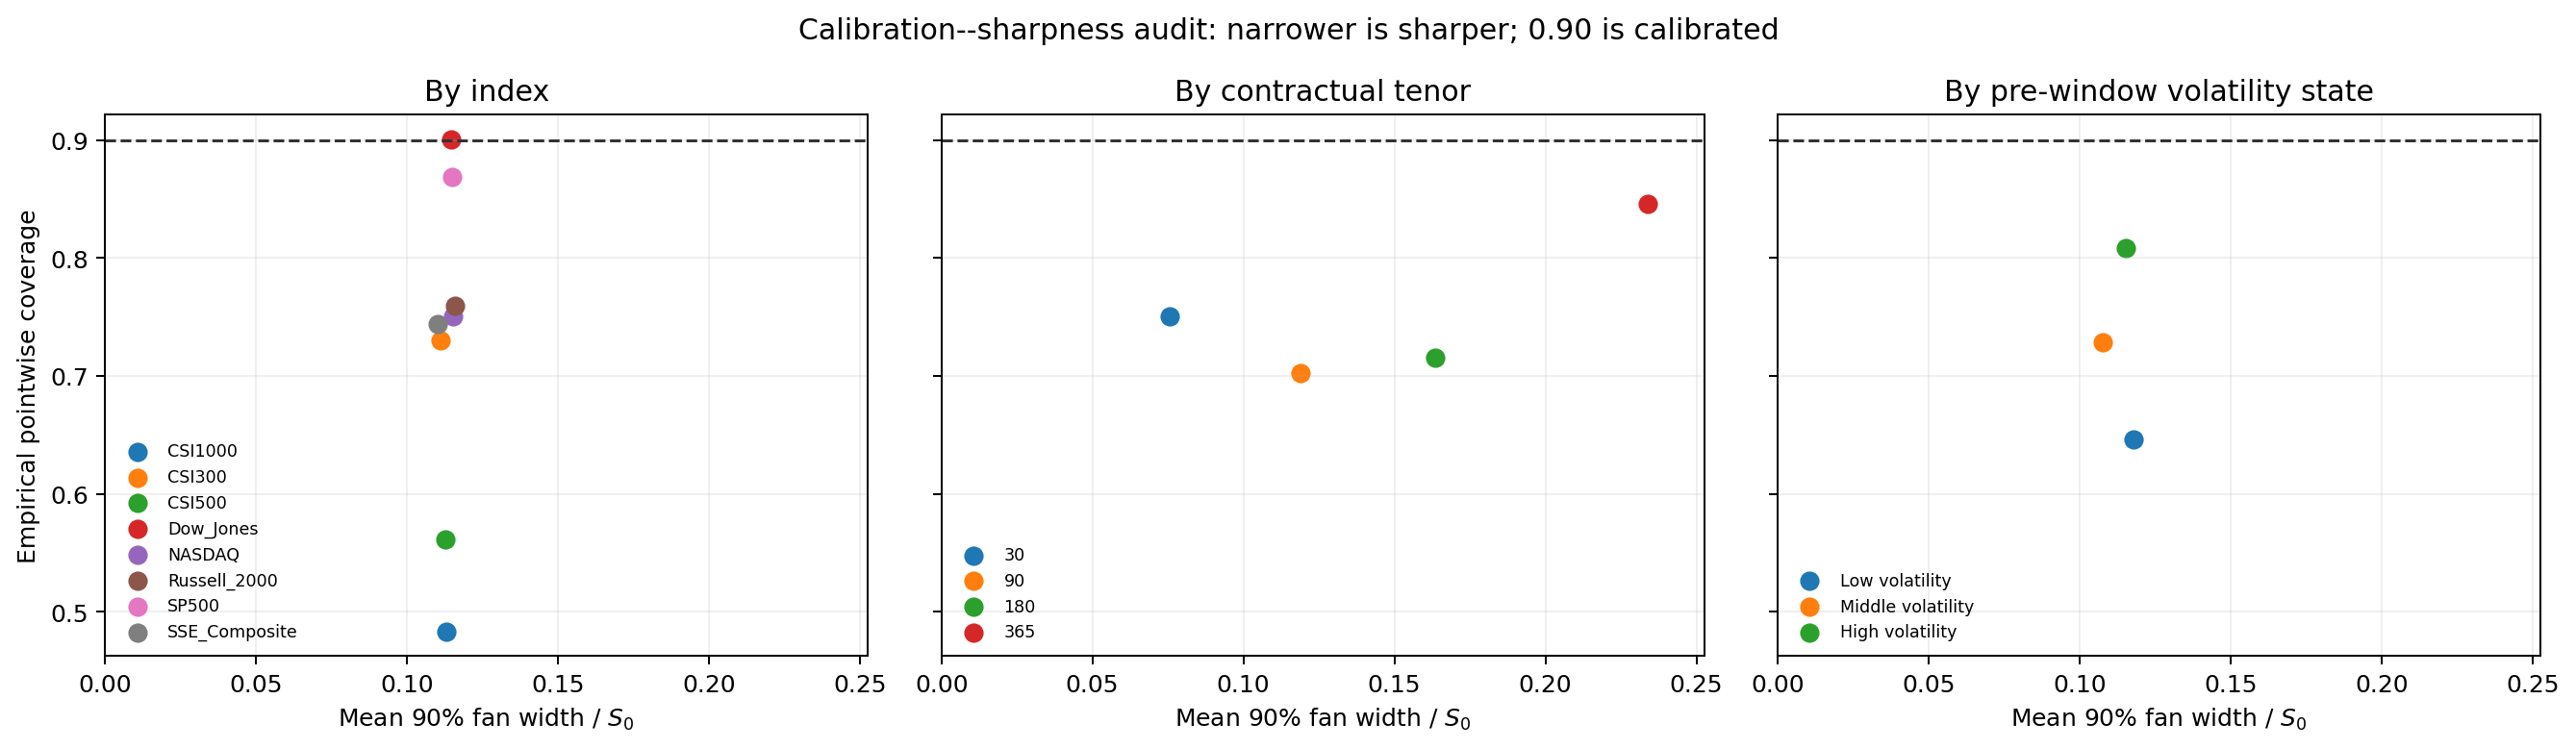
\includegraphics[width=\linewidth]{figures/final/05_calibration_sharpness.png}
\caption{Calibration--sharpness diagram for the central 90\% pointwise path
fan. Moving left indicates sharper intervals; moving toward the dashed 0.90
line indicates better calibration. Wide intervals with high coverage are not
automatically preferable, because the interval score penalizes excess width.}
\label{fig:calibration-sharpness}
\end{figure}

\begin{table}[p]
\singlespacing
\centering
\caption{Pointwise 90\% fan calibration by index, tenor, and pre-window state}
\label{tab:calibration-groups}
\resizebox{0.88\textwidth}{!}{%
\begin{tabular}{llrrr}
\toprule
Dimension & Group & Windows & Coverage & Mean width/$S_0$ \\
\midrule
Index & CSI 1000 & 827 & 0.4834 & 0.1129 \\
Index & CSI 300 & 827 & 0.7304 & 0.1111 \\
Index & CSI 500 & 827 & 0.5612 & 0.1127 \\
Index & Dow Jones & 879 & 0.9008 & 0.1146 \\
Index & NASDAQ & 879 & 0.7502 & 0.1153 \\
Index & Russell 2000 & 879 & 0.7594 & 0.1159 \\
Index & S\&P 500 & 879 & 0.8688 & 0.1150 \\
Index & SSE Composite & 827 & 0.7439 & 0.1102 \\
\midrule
Tenor & 30 days & 2{,}796 & 0.7507 & 0.0756 \\
Tenor & 90 days & 2{,}316 & 0.7025 & 0.1188 \\
Tenor & 180 days & 1{,}596 & 0.7154 & 0.1635 \\
Tenor & 365 days & 116 & 0.8457 & 0.2339 \\
\midrule
Trend & Low & 2{,}270 & 0.6394 & 0.1131 \\
Trend & Middle & 2{,}280 & 0.7694 & 0.1130 \\
Trend & High & 2{,}274 & 0.7740 & 0.1145 \\
\midrule
Drawdown & Deep & 2{,}276 & 0.6450 & 0.1117 \\
Drawdown & Middle & 2{,}274 & 0.7671 & 0.1133 \\
Drawdown & Shallow & 2{,}274 & 0.7710 & 0.1155 \\
\midrule
Volatility & Low & 2{,}272 & 0.6458 & 0.1178 \\
Volatility & Middle & 2{,}277 & 0.7288 & 0.1077 \\
Volatility & High & 2{,}275 & 0.8083 & 0.1151 \\
\bottomrule
\end{tabular}}
\tabnote{States are formed from information available before the forecast
window, using within-index terciles of 60-day trend, current drawdown, and
pre-window realized volatility. The machine-readable supplement also reports
terminal coverage, coverage error, and interval scores for every group.}
\end{table}

\begin{figure}[ht]
\centering
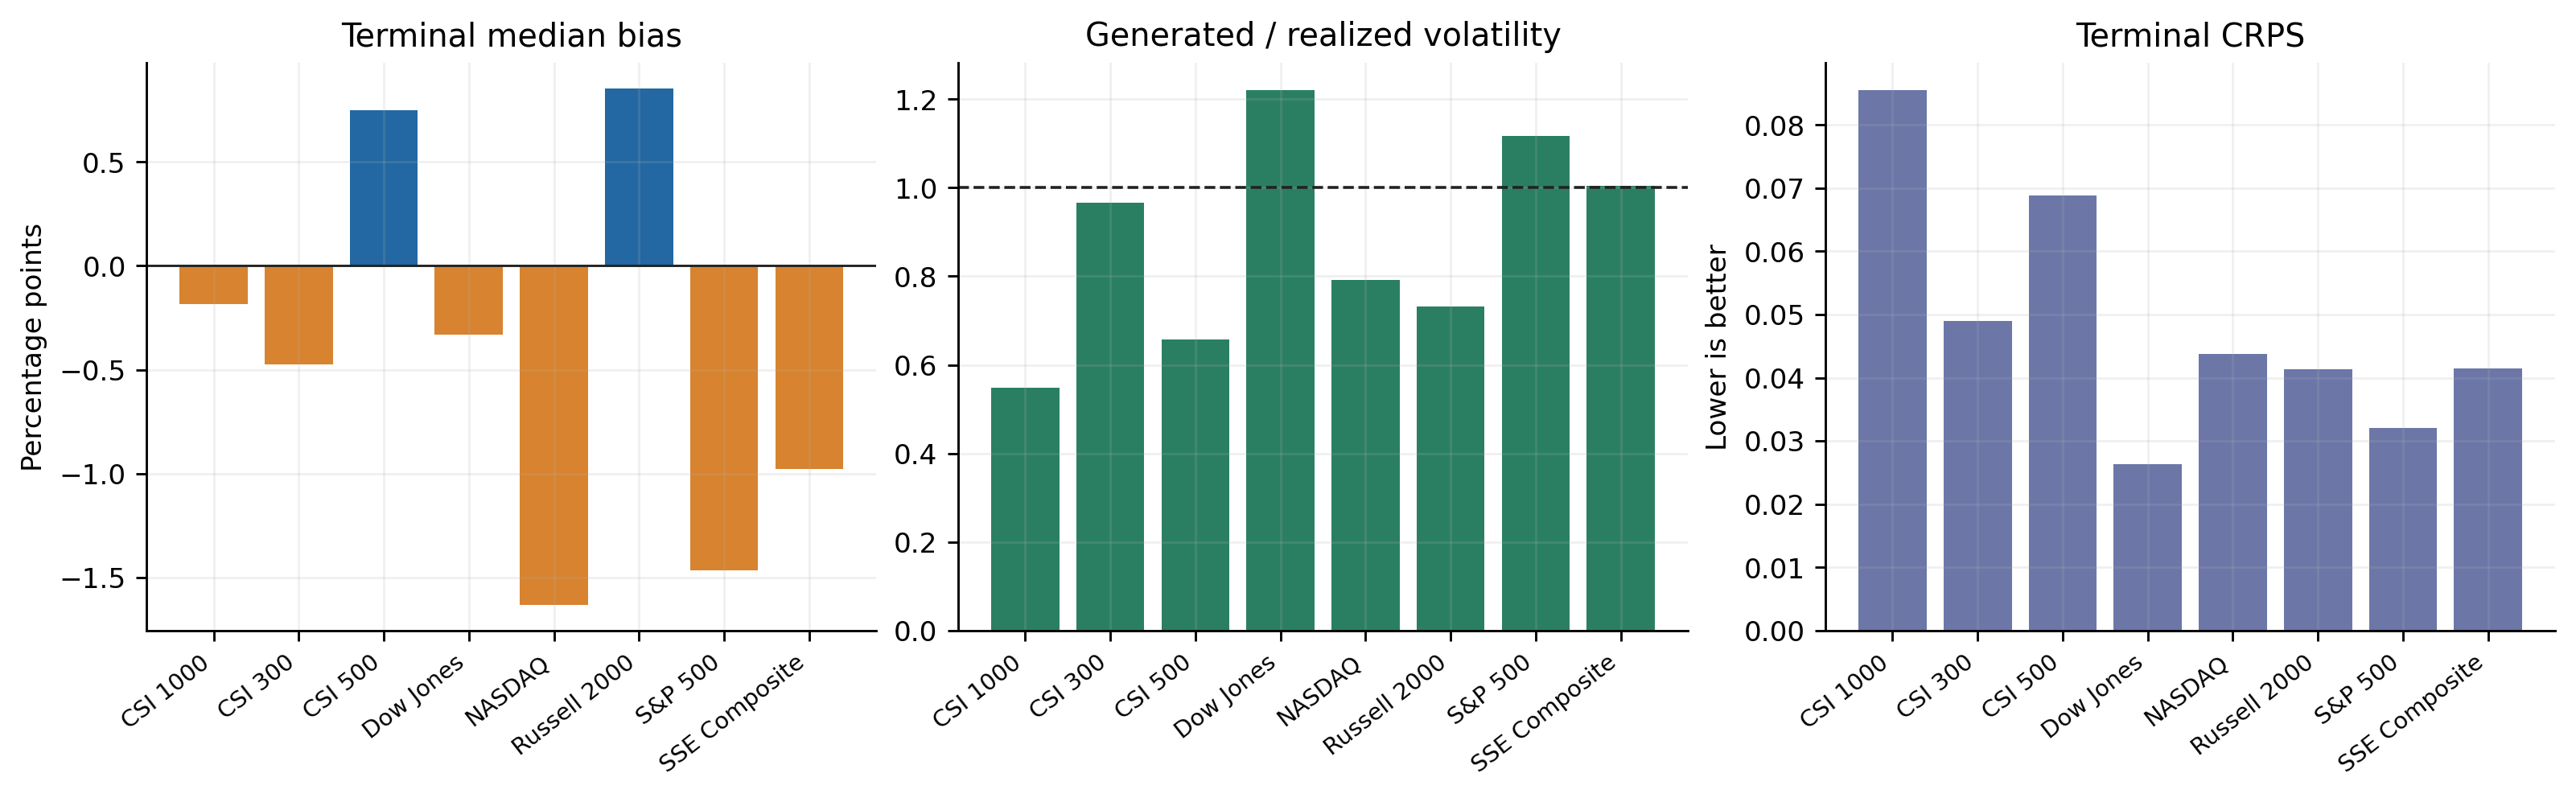
\includegraphics[width=\linewidth]{figures/final/02_path_quality_by_index.png}
\caption{Cross-index held-out path quality. The panels separate quantities
with different units and directions: terminal bias, volatility ratio, and
terminal CRPS are not placed on one common axis.}
\label{fig:pathquality}
\end{figure}

Figure~\ref{fig:pfans} shows one conditional fan per index. To avoid visual
cherry-picking, each panel uses the window at the median rank of absolute
terminal-median error for that index. The realized path begins at the same
observed $S_0$ as every generated path. The fans expand with horizon, change
scale across markets, and often place the realized trajectory close to the
conditional median. Sharp ex-post jumps can leave the central interval, as
they should in a probabilistic forecast; the relevant question is whether the
distribution assigns sensible mass around such events across the population,
which is measured in Table~\ref{tab:pathquality}.

\begin{figure}[p]
\centering
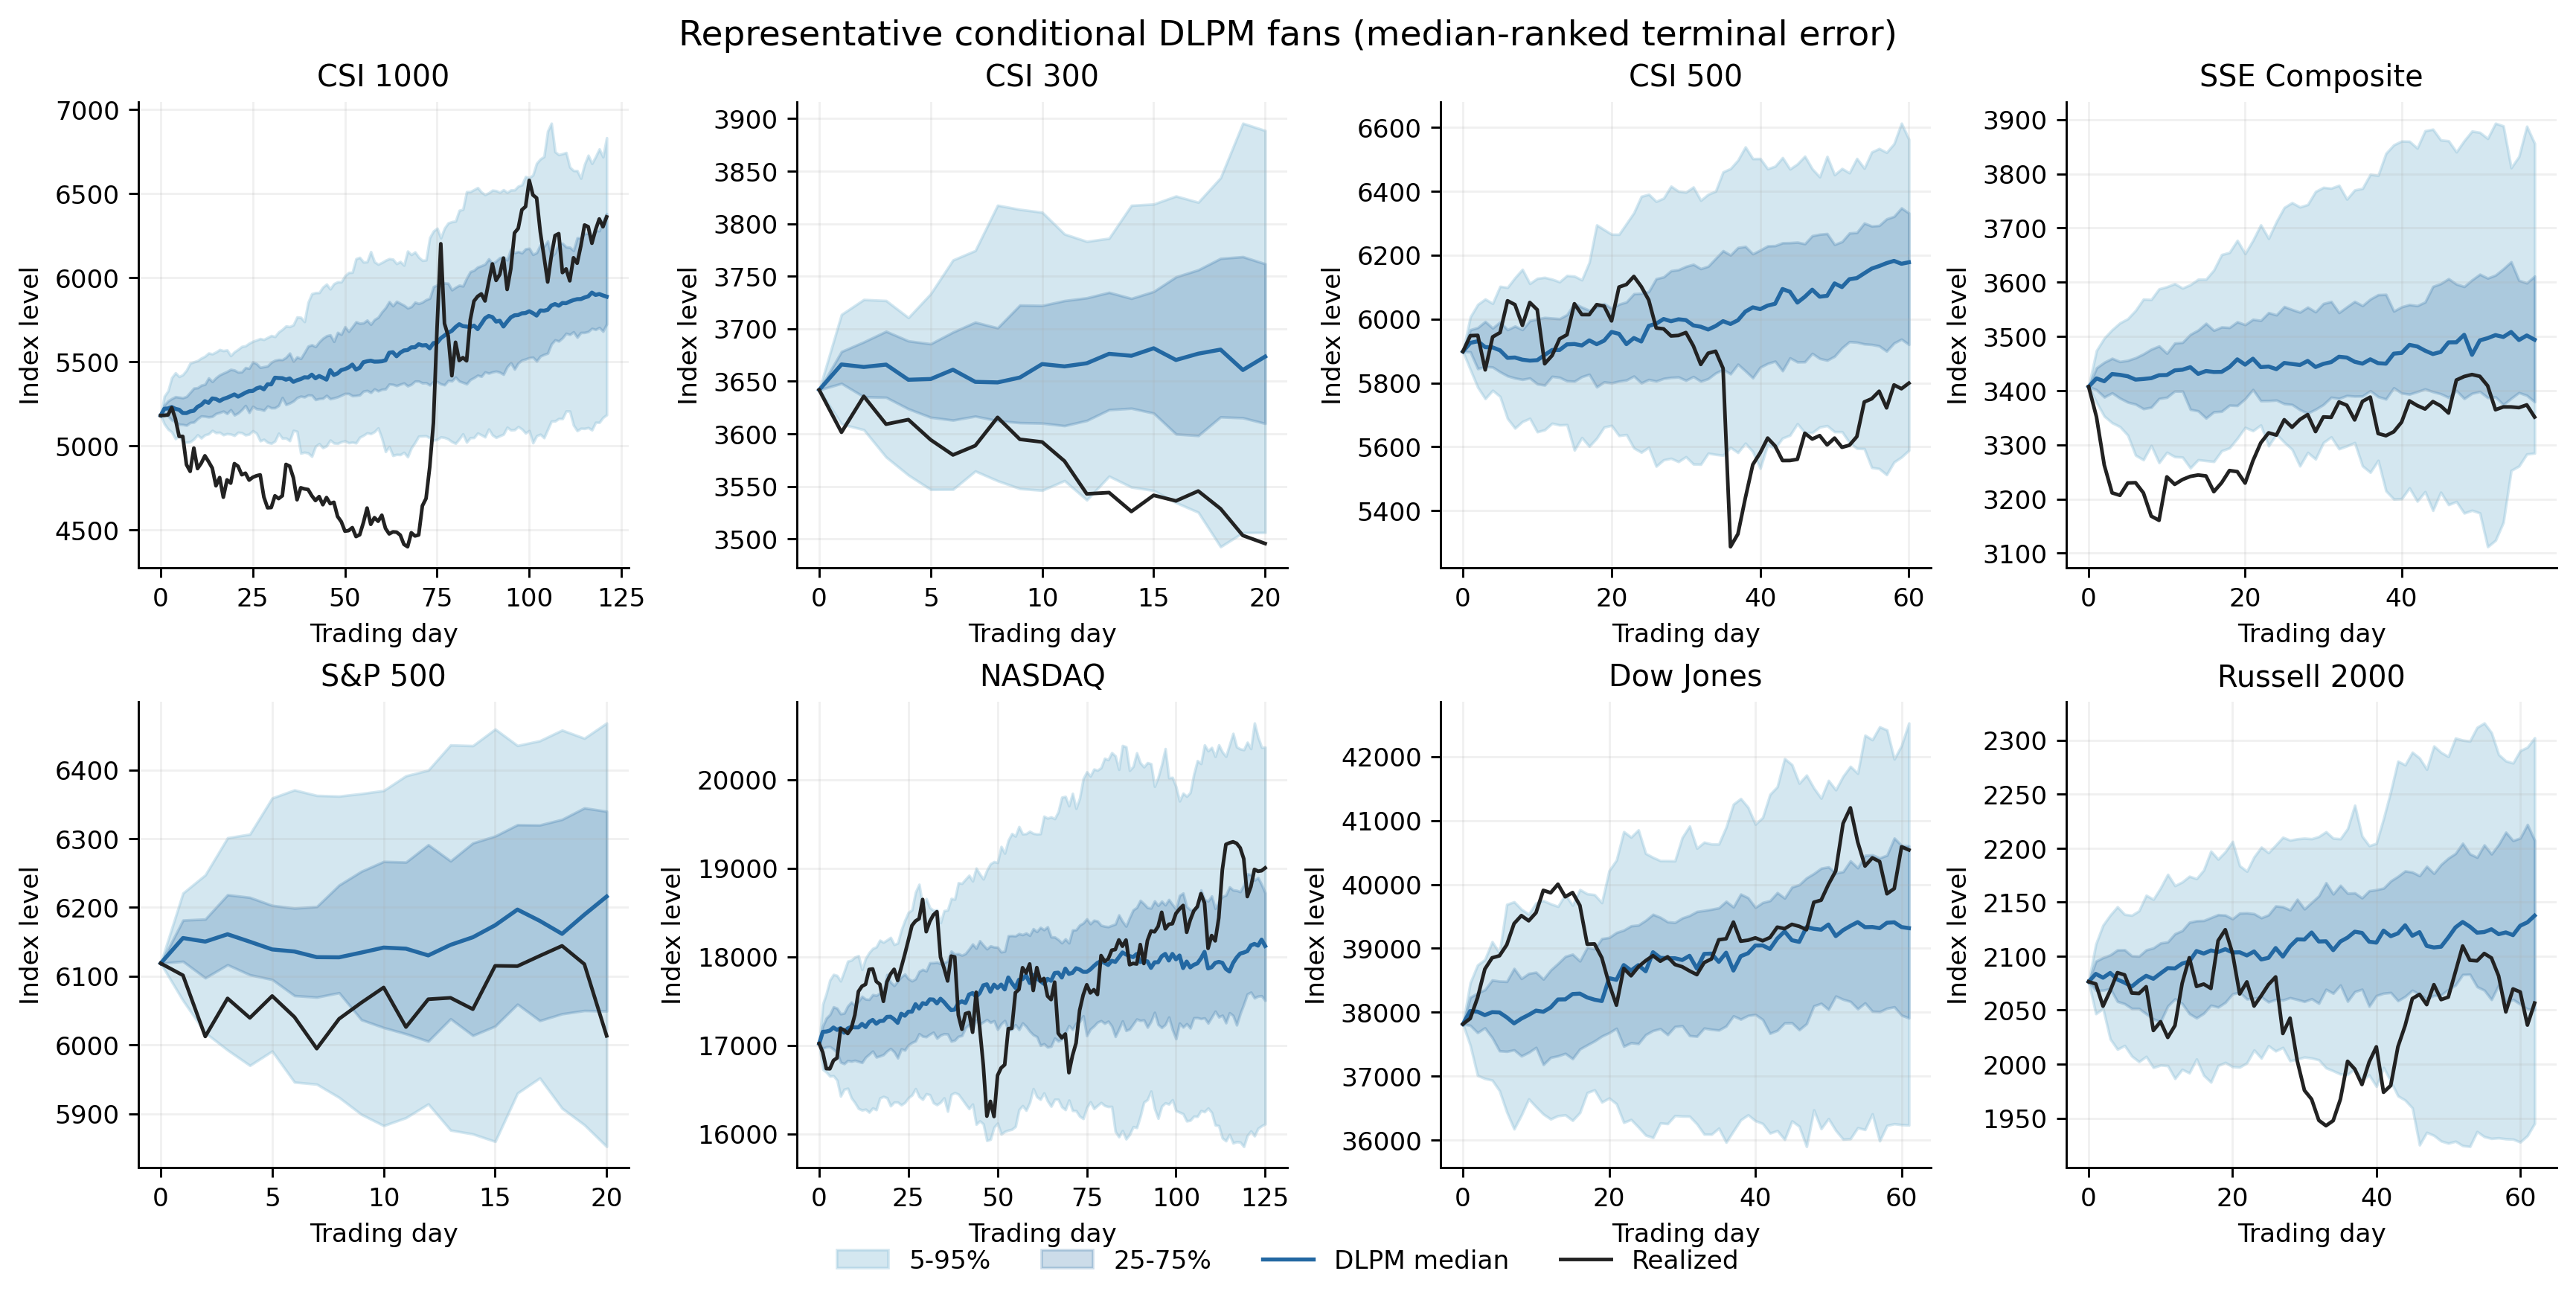
\includegraphics[width=\linewidth]{figures/final/03_p_only_fans_all_indices.png}
\caption{Representative DLPM-only conditional fans for all eight indices.
Panels are selected mechanically by median-ranked terminal error. Shading
shows 5--95\% and 25--75\% intervals; blue and black lines are the generated
median and held-out realization.}
\label{fig:pfans}
\end{figure}

\subsection{Interpreting center accuracy and uncertainty}

The audit separates aggregate level accuracy from conditional calibration.
Paths are exactly anchored at observed $S_0$, the signed drift error is small,
and the DLPM materially improves on the Gaussian controls. The interval
diagnostics provide a clear calibration target for deployment-specific
post-processing. The downstream P--Q experiment uses all generated paths as a
payoff-sensitivity diagnostic, complementing rather than replacing an
option-surface-calibrated workflow.

\subsection{Accelerated sampling}

The production sampler uses 50 DLIM steps rather than the complete 1{,}000-step
reverse chain. This makes the full 6{,}824-window, 40-path archive and repeated
payoff evaluation computationally feasible. Controlled sampler audits show
that acceleration changes higher moments more than the conditional center.
Accordingly, all headline statistical and economic numbers use the same
DLIM-50 archive; full-chain results are mechanism diagnostics, not silently
mixed into the game. This common-path discipline is more important than
choosing a sampler separately for every favorable metric.

\section{The Trader--Market-Maker P--Q Quoting Game}\label{sec:game}
\subsection{An independently constructed risk-neutral benchmark}

For each index, the Q benchmark begins with a Student-$t$ GARCH(1,1) volatility
recursion \citep{bollerslev1986garch},
\begin{align}
h_{t+1} &= \omega+\alpha \epsilon_t^2+\beta h_t,\\
z_{t+1} &\sim t_\nu,\qquad \epsilon_{t+1}=\sqrt{h_{t+1}}z_{t+1}.
\end{align}
Parameters are fitted to a deduplicated chronological return series through
the validation period. GARCH persistence and Student-$t$ tails make this a
materially stronger opponent than constant-volatility GBM.

Historical GARCH fitting does not itself define Q. We therefore transform the
innovation law and conditional drift explicitly. Let $z$ denote a standardized
Student-$t$ draw. A symmetric raw cap is solved so that, after truncation and
re-standardization,
\begin{equation}
\widetilde z
=\frac{\operatorname{clip}(z,-c_\nu,c_\nu)}
{\sqrt{\operatorname{Var}[\operatorname{clip}(z,-c_\nu,c_\nu)]}},
\qquad |\widetilde z|\leq 8,\qquad
\operatorname{Var}(\widetilde z)=1.
\end{equation}
This step is important: without post-truncation normalization, the simulated
innovation variance could be far below the fitted GARCH conditional variance
for low effective degrees of freedom.

The GARCH model is fitted to daily log returns (temporarily expressed in
percentage points for numerical estimation and converted back afterward).
Accordingly, $h_{t+1}$ is a one-trading-day conditional log-return variance,
not an annualized variance. For annualized risk-free rate $r_t$, annualized
dividend or carry yield $q_t$, and $\Delta=1/252$, define
\begin{equation}
\kappa_t=\log\mathbb E\left[
\exp\left(\sqrt{h_{t+1}}\,\widetilde z_{t+1}\right)
\mid\mathcal F_t\right].
\end{equation}
The RN-Q level process is
\begin{equation}
S_{t+1}=S_t\exp\left((r_t-q_t)\Delta-\kappa_t+
\sqrt{h_{t+1}}\,\widetilde z_{t+1}\right).
\label{eq:rnq}
\end{equation}
By construction,
\begin{equation}
\mathbb E^Q[e^{-(r_t-q_t)\Delta}S_{t+1}\mid\mathcal F_t]=S_t.
\end{equation}
The log-mgf is evaluated numerically under the same capped,
unit-variance innovation law used for simulation. Empirical audits across all
indices and 20-, 60-, 120-, and 240-day horizons produce mean discounted-price
ratios close to one.

The archived experiment sets $q_t=0$. All eight underlyings are observed as
price-index level series, but the conditioning data do not contain a matched
dividend-yield or futures-basis series. RN-Q is therefore an internally
risk-neutral, zero-carry benchmark under its specified law, rather than a
market-calibrated index-option measure. The code exposes $q_t$ explicitly for
future carry-aware experiments. A market-implied Q would additionally require
dividend or futures data and option-surface calibration. This qualification
does not alter the present martingale audit, which tests the stated $q_t=0$
benchmark.

\subsection{Why the comparison is informative}

P and Q encode different information. The DLPM learns a flexible,
history-conditioned physical distribution with heavy-tailed diffusion noise.
RN-Q imposes a discounted martingale while carrying GARCH volatility
persistence and Student-$t$ innovations. Comparing their payoff expectations
therefore asks whether information learned under P survives a disciplined,
nontrivial quoting benchmark.

For payoff $H(S_{0:T})$, define
\begin{align}
V_P &= e^{-rT}\mathbb E_P[H(S_{0:T})],\\
V_Q &= e^{-rT}\mathbb E_Q[H(S_{0:T})].
\end{align}
Price-level products use the symmetric total spread parameter $g$,
\begin{equation}
V_Q^{ask}=V_Q(1+g/2),\qquad
V_Q^{bid}=V_Q(1-g/2).
\label{eq:spread}
\end{equation}
Thus $g=0.10$ denotes a total 10\% bid--ask band, or approximately 5\% on
each side; it is not a 10\% transaction cost and not a guaranteed Q profit
rate. Structured rate-style products map the same stress parameter into their
documented notional-rate spread conventions.

The materiality threshold is stated in economically comparable spot units:
$\tau_S=0.01$. The P side buys when $V_P-V_Q^{ask}>\tau_S S_0$ and sells when
$V_Q^{bid}-V_P>\tau_S S_0$. If the realized discounted payoff is
$V_{\mathrm{real}}$, then
\begin{equation}
\mathrm{P\&L}=
\begin{cases}
V_{\mathrm{real}}-V_Q^{ask}, & \text{P buys},\\
V_Q^{bid}-V_{\mathrm{real}}, & \text{P sells},\\
0, & \text{no trade}.
\end{cases}
\end{equation}
The $1\%S_0$ threshold filters economically immaterial valuation gaps and is
separate from $g$. There is no additional hidden transaction-cost deduction in
the current experiment.

Because quotes are Monte Carlo estimates, we also report a sampling-aware
execution rule. For side-specific discounted payoff samples, let
$\widehat{\mathrm{SE}}_P$ and $\widehat{\mathrm{SE}}_Q$ denote the sample
standard deviation divided by the square root of the number of paths. A quote
passes the conservative filter only if
\begin{equation}
|V_P-V_Q^{\mathrm{side}}|>\tau_S S_0
+k\sqrt{\widehat{\mathrm{SE}}_P^2+\widehat{\mathrm{SE}}_Q^2}.
\label{eq:mcfilter}
\end{equation}
The primary table retains the economically transparent $k=0$ rule; $k=1$ and
$k=1.96$ are pre-specified robustness filters against threshold crossing caused
by quote noise.

\subsection{Final payoff protocol and alignment audit}

The final economic audit uses vanilla, arithmetic-average Asian, and
floating-strike lookback calls. These standard payoff families provide a
progression from terminal to average and running-extremum dependence while
remaining naturally comparable after normalization by initial spot. For each held-out contract window, the frozen
history-aware DLPM supplies 40 P paths and the independently calibrated RN-Q
benchmark supplies 256 paths. P and Q arrays are joined by
asset and chronological window identifier; file-level checks verify $S_0$,
rate, tenor, and realized future path before payoff evaluation. Results include
every window: a non-executed quote contributes zero P\&L. This unconditional
convention avoids the selection effect that occurs when results are averaged
only over executed trades.

For reproducibility, let a window contain the observed initial level and all
available subsequent trading-day observations,
$S_{0:m}=(S_0,S_1,\ldots,S_m)$, where $m$ is the stored
\texttt{actual\_trading\_days}; no unavailable date is padded. All three
standard contracts are at the money, $K=S_0$, and use
\begin{align}
H_{\mathrm{Vanilla}}(S_{0:m})
  &= (S_m-K)^+,\\
H_{\mathrm{Asian}}(S_{0:m})
  &= \left(\frac{1}{m+1}\sum_{i=0}^{m}S_i-K\right)^+,\\
H_{\mathrm{Lookback}}(S_{0:m})
  &= \left(S_m-\min_{0\le i\le m}S_i\right)^+.
\end{align}
The quoted value is $e^{-r m/252}$ times the Monte Carlo mean payoff, using
the annualized window rate $r$. The initial RN-Q Delta diagnostic uses a
central spot bump $\epsilon=0.001$,
\begin{equation}
\Delta_0=\frac{V_Q(S_0(1+\epsilon))-V_Q(S_0(1-\epsilon))}
{2\epsilon S_0},
\end{equation}
with common random numbers: the same RN-Q innovations are rescaled under both
spot bumps. The resulting index position is opened once and held to maturity;
it is not a dynamic replication strategy.

\subsection{Structured-product stress-test scenarios}

The scope of the paper extends beyond smooth options. We retain two explicitly
specified structured-product scenarios as stress tests for future P--Q
evaluation: an accumulator and a snowball/autocall note. Their purpose is not
to produce a single number comparable with a vanilla option price. Rather, they
expose the generated path distribution to repeated observations, early
termination, leverage after a drawdown, and clustered tail events---the
features for which a terminal marginal is least informative.

\begin{table}[ht]
\singlespacing
\centering
\caption{Structured-product stress-test specifications}
\label{tab:structured-scenarios}
\begin{tabular}{p{0.22\linewidth}p{0.67\linewidth}}
\toprule
Scenario & Frozen payoff convention \\
\midrule
Accumulator & Daily observations; purchase strike $0.85S_0$; knock-out at
$1.05S_0$; two-times quantity below strike; scheduled payoff normalized by
the number of remaining observations. \\
Snowball/autocall & Five-day knock-out observations at $1.05S_0$; knock-in
barrier $0.80S_0$; annual coupon rate 15\%; maturity loss conditional on a
knock-in without knock-out. \\
\bottomrule
\end{tabular}
\tabnote{These are scenario specifications, not smooth-option price-equivalent
contracts. A valid empirical report must separately state coupon and loss
distributions, knock-in and knock-out frequencies, expected shortfall after
knock-in, and Monte Carlo concentration. They are therefore not pooled with
the normalized Vanilla/Asian P\&L headline table.}
\end{table}

The mean quote standard errors, normalized by $S_0$, are 0.66\%, 0.38\%, and
0.63\% on the P side and 0.39\%, 0.20\%, and 0.41\% on the Q side for Vanilla,
Asian, and Lookback, respectively. Table~\ref{tab:mcfilter} therefore subjects
the result to the explicit measurement-error filter in
Equation~\eqref{eq:mcfilter}. The stricter rules sharply reduce execution, as
they should, while the unconditional Vanilla and Lookback diagnostics remain
positive.

\begin{table}[ht]
\singlespacing
\centering
\caption{Monte Carlo quote-uncertainty audit at $g=0.05$ and $\tau_S=1\%S_0$}
\label{tab:mcfilter}
\begin{tabular}{llrr}
\toprule
Filter & Contract & Trade rate & Unconditional P\&L/$S_0$ \\
\midrule
$k=0$ & Vanilla / Asian / Lookback & 30.95\% / 13.69\% / 35.04\% & 0.91\% / 0.36\% / 0.28\% \\
$k=1$ & Vanilla / Asian / Lookback & 11.24\% / 4.35\% / 14.63\% & 0.44\% / 0.12\% / 0.17\% \\
$k=1.96$ & Vanilla / Asian / Lookback & 4.05\% / 1.64\% / 5.95\% & 0.25\% / 0.04\% / 0.08\% \\
\bottomrule
\end{tabular}
\tabnote{The filter adds $k$ joint Monte Carlo standard errors to the fixed
materiality threshold. P uses 40 paths and RN-Q uses 256 paths in every row.}
\end{table}

At the stringent $k=1.96$ setting, varying $\tau_S$ from 0.5\% to 1.0\% and
1.5\% changes the Vanilla trade rate from 7.44\% to 4.05\% and 2.51\%, with
unconditional P\&L of 0.34\%, 0.25\%, and 0.19\%. The corresponding Lookback
figures are 11.23\%, 5.95\%, and 2.95\% for execution and 0.11\%, 0.08\%, and
0.04\% for P\&L. Asian is more sensitive, falling from 0.10\% to 0.04\% and
approximately zero. Thus the smooth-option evidence is not based on an
unreported 40\% threshold, and its strongest residual is concentrated in
Vanilla and the running-extremum contract.

The present aligned economic archive reports the three standard contracts below.
The one-time delta check is reported only for Vanilla and Asian because a
static delta is not a complete hedge for a running-extremum payoff. The
structured scenarios are evaluated separately with the same unique-key P/Q
alignment. Table~\ref{tab:structured-results} reports normalized-notional
scenario statistics, not option prices. The P generator produces higher mean
scenario payoff than RN-Q for both products while retaining realistic
early-termination behavior: the realized accumulator mean lies below both
generated means, whereas the realized snowball mean lies between the P and Q
means; realized knock-out and coupon frequencies are
of the same order as both generated mechanisms.

\begin{table}[ht]
\singlespacing
\centering
\caption{Aligned structured-product scenario audit on 6{,}824 windows}
\label{tab:structured-results}
\resizebox{\linewidth}{!}{%
\begin{tabular}{lrrrrrr}
\toprule
Scenario & P mean & RN-Q mean & Realized mean & P--Q gap & P/Q/realized KO rate & P/Q/realized coupon rate \\
\midrule
\StructuredRows
\bottomrule
\end{tabular}}
\tabnote{Each figure is a normalized-notional scenario payoff or event
frequency. The reported P archive has 40 paths per window and RN-Q has 256.
Results are not combined with
the smooth-option P\&L table because the contracts have different economic
units and loss mechanisms.}
\end{table}

The positive mean and event-rate evidence makes these products useful
stress-test cases for a path generator, rather than merely background
examples. At the same time, the path-level tail audit finds that the current P
generator understates rare Snowball knock-ins relative to the realized panel.
Accordingly, the evidence supports structured-product scenario generation and
average-payoff diagnostics, but not yet standalone tail-risk pricing for
knock-in products.

The main dealer-spread point is $g=0.05$, with $g=0.10$ and $g=0.20$ reported
as pre-specified stress cases. All reported smooth-option diagnostics use the
same complete-window archive with 40 P paths per window.

\subsection{Final P--Q payoff results}

Table~\ref{tab:mainpnl} reports the final normalized results. The P and Q
archives are joined with the unique key (asset, start date, $S_0$, tenor,
rate), rather than by row position; the post-join initial-price check is exact
to numerical tolerance. At $g=0.05$ and $\tau_S=1\%S_0$, unconditional Vanilla
P\&L is 0.91\% of $S_0$ and Asian P\&L is 0.36\%. The associated execution
rates are 30.95\% and 13.69\%, respectively. Buy and sell directions are both
represented, but the positive raw gap is predominantly a buy-side contribution.
This motivates the drift-neutral and hedged counterfactuals below.

\begin{table}[ht]
\singlespacing
\centering
\caption{Final P--Q payoff diagnostic at $g=0.05$ and $\tau_S=1\%S_0$}
\label{tab:mainpnl}
\resizebox{\textwidth}{!}{%
\begin{tabular}{lrrrrrrrr}
\toprule
Contract & P\&L/$S_0$ & Trade rate & Win rate & P-buy share & Buy P\&L/$S_0$ & P-sell share & Sell P\&L/$S_0$ \\
\midrule
\MainPnlRows
\bottomrule
\end{tabular}
}
\tabnote{P\&L is unconditional across all 6{,}824 windows and normalized by
initial spot. A no-trade window contributes zero. Buy/sell shares condition on
an executed trade. Buy and sell P\&L columns are unconditional contributions:
trade rate $\times$ direction share among active trades $\times$ mean P\&L of
that direction; their sum equals total P\&L/$S_0$.}
\end{table}

The Lookback result is especially useful as a simple exotic diagnostic: it
depends on the running minimum rather than only a terminal or average level.
Its 66.12\% sell-side share is materially higher than for Vanilla and Asian,
so the positive unconditional value is not merely a long-trend signal. Because
the payoff depends on extrema, its sampling uncertainty is wider; it is
therefore reported alongside, rather than folded into, the static-delta table.

\begin{table}[ht]
\singlespacing
\centering
\caption{One-time RN-Q Delta-hedged payoff diagnostic at $g=0.05$ and $\tau_S=1\%S_0$}
\label{tab:hedged}
\begin{tabular}{lrrrr}
\toprule
Contract & Trade rate & Unhedged P\&L/$S_0$ & Hedged P\&L/$S_0$ & Hedged active win rate \\
\midrule
\HedgedRows
\bottomrule
\end{tabular}
\tabnote{An RN-Q central-difference Delta is set at inception and held to maturity.
This is a directional-exposure diagnostic, not a full dynamic hedge or a
transaction-cost-inclusive trading strategy.}
\end{table}

\begin{table}[ht]
\singlespacing
\centering
\caption{Dealer-spread sensitivity of unconditional normalized P\&L}
\label{tab:greed}
\begin{tabular}{lrrrrrr}
\toprule
& \multicolumn{2}{c}{$g=0.05$} & \multicolumn{2}{c}{$g=0.10$} &
\multicolumn{2}{c}{$g=0.20$} \\
\cmidrule(lr){2-3}\cmidrule(lr){4-5}\cmidrule(lr){6-7}
Contract & P\&L/$S_0$ & Trade & P\&L/$S_0$ & Trade & P\&L/$S_0$ & Trade \\
\midrule
\SpreadRows
\bottomrule
\end{tabular}
\tabnote{The parameter $g$ is the total symmetric dealer spread in
Equation~\eqref{eq:spread}, not a transaction-cost estimate.}
\end{table}

\subsection{Drift-neutral counterfactual and economic interpretation}

The P--Q diagnostic intentionally compares a learned physical distribution
with an independently constructed martingale benchmark. Its payoff gap
therefore contains several economically meaningful channels: physical
risk-premium exposure, state-dependent volatility and tail-shape differences,
and conditional path geometry. We decompose this gap with two conservative
counterfactuals. Terminal-drift neutralization moves Vanilla and Asian P\&L
from 0.91\% and 0.36\% to $-0.95\%$ and $-0.32\%$; a one-time initial RN-Q
delta hedge yields 0.33\% and $-0.04\%$. Thus physical direction exposure is
an important component of the raw P--Q gap. At the same time, the positive
static-hedged Vanilla residual shows that the selected conditional scenarios
retain a non-directional payoff component under this diagnostic. The Asian
residual is close to zero. This evidence is not used to select the model: the
P--Q module is a transparent payoff-sensitive stress test, with no option
price or downstream payoff entering DLPM training or checkpoint selection.

\subsection{Dependence-aware uncertainty}

We reconstruct P\&L for every asset--date--contract cell and jointly resample
common calendar blocks across all eight indices. This preserves cross-market
shocks and the serial overlap created by rolling windows. Table~\ref{tab:boot}
reports the $g=0.05$, $\tau_S=1\%S_0$ intervals. The 20- and 60-day blocks are primary;
90--150 days are medium-horizon checks. The 180- and 252-day entries use only
three effective blocks and are presented as long-dependence sensitivities.

\begin{table}[ht]
\singlespacing
\centering
\caption{Joint calendar-block bootstrap, unconditional P\&L/$S_0$ at $g=0.05$ and $\tau_S=1\%S_0$}
\label{tab:boot}
\resizebox{\textwidth}{!}{%
\begin{tabular}{rrrrrr}
\toprule
Block days & Effective blocks & Vanilla 95\% CI & Asian 95\% CI & Lookback 95\% CI & Role \\
\midrule
20 & 27 & [0.32\%, 1.55\%] & [0.08\%, 0.73\%] & [-0.02\%, 0.70\%] & Primary \\
60 & 9 & [0.10\%, 1.73\%] & [-0.03\%, 0.79\%] & [-0.06\%, 0.71\%] & Primary \\
90 & 6 & [0.01\%, 2.18\%] & [-0.04\%, 0.97\%] & [-0.14\%, 0.81\%] & Medium horizon \\
120 & 5 & [-0.02\%, 1.66\%] & [0.03\%, 0.70\%] & [-0.16\%, 0.76\%] & Medium horizon \\
150 & 4 & [0.00\%, 2.08\%] & [0.03\%, 0.84\%] & [-0.29\%, 1.11\%] & Medium horizon \\
180 & 3 & [0.11\%, 2.08\%] & [0.01\%, 0.95\%] & [-0.01\%, 0.90\%] & Long sensitivity \\
252 & 3 & [0.07\%, 1.04\%] & [-0.01\%, 0.40\%] & [0.33\%, 0.41\%] & Long sensitivity \\
\bottomrule
\end{tabular}}
\tabnote{Each interval uses 2{,}000 joint calendar-block replications. The
long-block results should not be treated as decisive because the effective
number of blocks is small. Intervals are calculated from $S_0$-normalized
window P\&L, so indices have equal economic weight rather than being weighted
by their index level.}
\end{table}

\subsection{State-conditional comparison}

The pooled bootstrap comparison is intentionally retained as a demanding
nonparametric control: resampling reuses realized historical moves and is
therefore naturally strong on unconditional marginal diagnostics. It cannot,
however, distinguish a quiet start from a trend reversal or a drawdown. Since
the central DLPM claim is conditional generation, Table~\ref{tab:regime-crps}
stratifies the same frozen test set using pre-window, within-index terciles.
The DLPM has lower point-estimate terminal CRPS in low-trend and deep-drawdown
states, the two settings in which conditional path stress testing is most
consequential. Against unconditional resampling these small paired differences
are descriptive: joint calendar-block intervals cross zero and Holm-adjusted
$p$-values across the six pre-specified state slices equal one. This motivates
the more direct state-matched counterfactual reported next.

\begin{table}[ht]
\singlespacing
\centering
\caption{Regime-stratified terminal CRPS: frozen DLPM versus historical block bootstrap}
\label{tab:regime-crps}
\resizebox{\textwidth}{!}{%
\begin{tabular}{lrrr}
\toprule
Pre-window state (within-index tercile) & Windows & DLPM CRPS & Bootstrap CRPS \\
\midrule
Low 60-day trend & 2{,}270 & 0.06464 & 0.06562 \\
Middle 60-day trend & 2{,}280 & 0.04455 & 0.04355 \\
High 60-day trend & 2{,}274 & 0.03639 & 0.03671 \\
Deep current drawdown & 2{,}276 & 0.06044 & 0.06194 \\
Middle current drawdown & 2{,}274 & 0.04316 & 0.04342 \\
Shallow current drawdown & 2{,}274 & 0.04192 & 0.04047 \\
\bottomrule
\end{tabular}}
\tabnote{Lower CRPS is better. Regimes are formed from information observable
at the contract start, separately within each index. Relative DLPM improvements
are 1.49\% in low-trend and 2.41\% in deep-drawdown windows. Historical block
resampling has a mechanical advantage for linear trend continuation because it
directly reuses realized trend blocks; nevertheless, the DLPM remains
competitive in high-trend windows and is more informative in stress states
where the pre-window volatility, drawdown, and reversal context matters. The
paired state-slice differences are not statistically distinguishable after
joint calendar-block resampling and Holm correction. This table compares
against an unconditional replay mechanism; it does not test the direct
state-matched counterfactual in Table~\ref{tab:state-matched}.}
\end{table}

Motivated by conditional predictive-ability evaluation
\citep{giacomini2006conditional}, we test the paper's conditional claim with a
separate, no-training state-matched empirical control. Its construction was
specified without observing target paths: for each test window it selects the
40 nearest training windows with the same index and contractual tenor, using
only standardized pre-window 60-day realized volatility, trend, and current
drawdown. It never observes the test target. Table~\ref{tab:state-matched}
shows that the DLPM lowers aggregate CRPS by 23.3\%; the paired difference is
negative at every joint calendar-block length from 20 through 150 days.

\begin{table}[ht]
\singlespacing
\centering
\caption{Terminal CRPS against the state-matched empirical control}
\label{tab:state-matched}
\resizebox{\textwidth}{!}{%
\begin{tabular}{lrrr}
\toprule
Slice & Windows & DLPM CRPS & State-matched CRPS \\
\midrule
All windows & 6{,}824 & 0.04851 & 0.06329 \\
Low / middle / high trend & 2{,}270 / 2{,}280 / 2{,}274 & 0.06464 / 0.04455 / 0.03639 & 0.08368 / 0.05244 / 0.05380 \\
Deep / middle / shallow drawdown & 2{,}276 / 2{,}274 / 2{,}274 & 0.06044 / 0.04316 / 0.04192 & 0.07826 / 0.05667 / 0.05491 \\
China / United States & 3{,}308 / 3{,}516 & 0.06156 / 0.03624 & 0.08279 / 0.04494 \\
\bottomrule
\end{tabular}}
\tabnote{Lower is better. The overall DLPM-minus-control difference is
$-0.01477$. The 95\% joint calendar-block intervals are
$[-0.01760,-0.00727]$ at 20 days, $[-0.01878,-0.00475]$ at 60 days,
$[-0.02111,-0.00239]$ at 90 days, $[-0.01928,-0.00320]$ at 120 days, and
$[-0.01759,-0.00344]$ at 150 days (2{,}000 replications).}
\end{table}

\begin{figure}[ht]
\centering
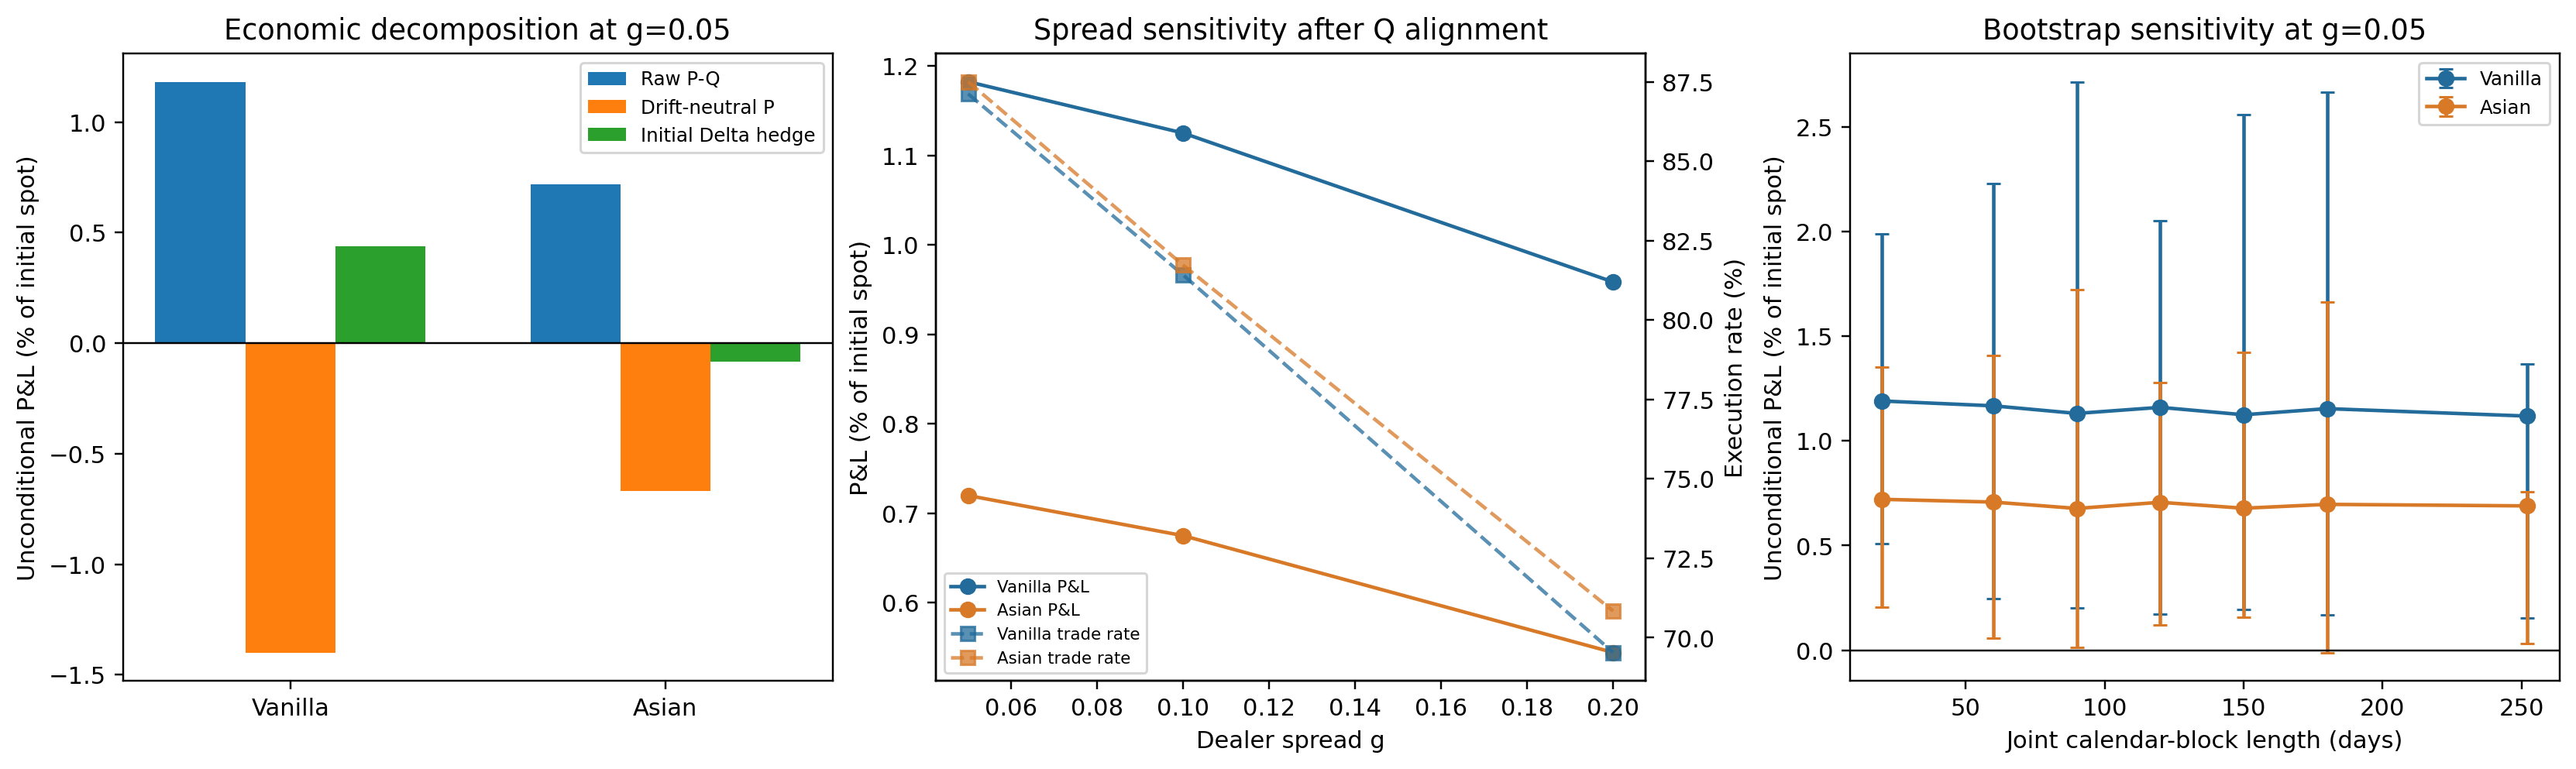
\includegraphics[width=0.92\linewidth]{figures/final/04_aligned_economic_audit.png}
\caption{Aligned economic audit. The first panel separates the raw P--Q
diagnostic from terminal-drift-neutral and one-time initial-delta-hedged
counterfactuals. The remaining panels show dealer-spread sensitivity and
dependence-aware bootstrap intervals. All displayed P\&L values are
unconditional and normalized by initial spot.}
\label{fig:aligned-econ}
\end{figure}

\section{Limitations and Scope}\label{sec:limitations}
Six boundaries qualify the reported results; each is stated where it arises
and consolidated here. First, the deployed sampler is numerically truncated:
auxiliary draws are capped at $a_t \le 100$ and coordinate-wise innovations
at $\lvert\varepsilon\rvert \le 2$, so every reported statistic describes an
effective, finite-support heavy-tailed process rather than an unbounded
stable law (Section~\ref{sec:dlpm}, Table~\ref{tab:tails}). Second, the
generator is under-dispersed at the pooled level: overall pointwise fan
coverage is 0.7277 against a 0.90 target, with the shortfall concentrated in
CSI~1000, CSI~500, and low-trend, deep-drawdown, low-volatility windows;
because fan width varies far less than coverage across these groups, a single
global widening factor would over-widen already calibrated markets, and
state-dependent conditional-width calibration is the identified frontier.
Third, the two Gaussian diffusion controls share the backbone and
conditioning but use a separately implemented auxiliary-loss stack; since
$\alpha = 2$ recovers the Gaussian chain exactly within the DLPM
parameterization, a fully budget- and loss-matched $\alpha$-ablation is the
cleanest isolation of the heavy-tailed mechanism's marginal contribution and
is left to future work. Fourth, the RN-Q benchmark is an internally
consistent zero-carry construction: no option-surface, dividend, or
futures-basis information enters the audit, so P--Q values measure
disagreement with a stated benchmark law rather than mispricing against
market quotes. Fifth, the economic results are belief-based diagnostics under
pre-specified spread and materiality conventions, not
transaction-cost-inclusive trading claims; joint calendar-block intervals for
the Asian and Lookback contracts cross zero at several block lengths
(Table~\ref{tab:boot}). Sixth, the structured-product module supports
scenario generation and average-payoff diagnostics but not standalone
tail-risk pricing for knock-in products, whose rare-event frequencies remain
understated relative to the realized panel.

\section{Conclusion}\label{sec:conclusion}
This paper develops a history-aware financial adaptation of Denoising L\'evy
Probabilistic Models for conditional path generation and evaluates it under a
broad, chronology-respecting
cross-market protocol. The contribution is theoretical, computational, and
empirical: it combines an $\alpha$-stable diffusion mechanism with a U-Net
conditioned on long return histories and financial state variables, and it
evaluates one frozen generator over 6{,}824 out-of-time windows from eight
Chinese and U.S. indices.

The final audit supports a substantive contribution. The history-aware DLPM
improves terminal CRPS from 0.0548 for contract-only DLPM and 0.0831 for the
simple Gaussian diffusion control to 0.0485, with path energy score 0.3368,
generated-to-realized volatility ratio 0.882, and an aggregate signed
terminal-median bias of $-0.46$pp. These gains arise from a single global
model spanning eight Chinese and U.S. indices, long historical conditioning,
state-aware sampling weights, and a heavy-tailed diffusion mechanism. The
effective-tail audit locates the mechanism's contribution within its
numerical support: generated first-step returns reproduce the realized
left-tail-to-IQR ratio almost exactly (2.91 versus 2.93) with similar
two-sided Hill decay, while remaining narrower than realized returns in
absolute exceedance---the same under-dispersion that the calibration audit
localizes to specific indices and pre-window states.

The conditional comparison sharpens the interpretation of the bootstrap
result. Unconditional historical resampling is deliberately difficult to beat
on pooled marginal statistics because it directly reuses realized return
blocks; its overall paired CRPS difference from DLPM is statistically
indistinguishable from zero. The more relevant state-matched empirical control
uses the same index, tenor, volatility, trend, and drawdown information but no
neural generator. Against that direct counterfactual, DLPM reduces terminal
CRPS from 0.0633 to 0.0485, a 23.3\% improvement, with joint calendar-block
intervals excluding zero at 20, 60, 90, 120, and 150 days. This identifies the
value of learning a continuous conditional path law rather than merely
replaying nearby historical states.

The downstream P--Q audit complements, rather than validates, the path
diagnostics. At $g=0.05$ and $\tau_S=1\%S_0$, raw unconditional P\&L is
0.91\% of spot for Vanilla, 0.36\% for Asian, and 0.28\% for floating-strike
Lookback calls. Lookback is a particularly useful simple-exotic check because
its payoff depends on a running extremum and its positive result contains a
majority sell-side contribution. The one-time RN-Q Delta-hedged diagnostic
retains 0.33\% for Vanilla while Asian is close to zero at -0.04\%.
Terminal-drift-neutral counterfactuals show that physical direction remains an
important component of the raw values. The aligned Accumulator and Snowball
scenarios provide a demanding test of payoff, knock-out, and knock-in
mechanics; they are reported as risk scenarios rather than as static-hedge
trading claims. This makes the payoff module more informative than a single
unqualified backtest without conflating P--Q disagreement with economic alpha.
An explicit quote-error audit further shows that adding one joint Monte Carlo
standard error to the 1\% materiality threshold leaves positive unconditional
P\&L of 0.44\%, 0.12\%, and 0.17\% for Vanilla, Asian, and Lookback, while
reducing execution to 11.24\%, 4.35\%, and 14.63\%. The economic module thus
documents payoff relevance under conservative selection without serving as
the model-selection criterion.

The resulting framework is useful for conditional scenario generation,
cross-market stress testing, payoff-sensitive structured-product analysis, and
belief-based derivative research. Future work can extend the same engineering
stack with conditional-width calibration, sampler distillation, and a direct
connection between the physical generator and an option-surface-calibrated
market Q.

\section*{Funding}
No funding was obtained for this work.

\section*{Disclosure statement}
The authors report there are no competing interests to declare.

\section*{Data availability statement}
The implementation, frozen experiment configuration, audit scripts, and the
compact result data underlying all tables and figures in this article are
openly available in the companion repository at
\url{https://github.com/Junchi-Shen/DLPM}. Large binary artifacts, including
model checkpoints and generated path archives, are archived on Hugging Face
at \url{https://huggingface.co/Islandshen/DLPM}. Raw market index series
were obtained from public providers (AKShare for the Chinese indices and
Yahoo Finance for the U.S. indices) and remain subject to those providers'
redistribution terms; the repository documents the tickers, transformations,
and chronological split boundaries required to rebuild the experimental
panel from the original sources.

\section*{Declaration of generative AI use}
During the preparation of this work the authors used generative AI coding
and editing assistants (OpenAI Codex and Anthropic Claude Code, 2025--2026
releases) to assist with software implementation, experiment tooling, and
language editing. All research design, model specifications, analyses,
results, and conclusions are the authors' own; the authors reviewed and
verified all generated content and take full responsibility for the
content of this manuscript.

\appendix


\section{Network Architecture}\label{app:architecture}

\paragraph{Backbone.} We use a one-dimensional conditional U-Net
\citep{ronneberger2015unet} with base width 64, channel multipliers
$(1, 2, 4, 8)$, dropout 0.1, and 17.0 million parameters. The encoder
consists of residual convolutional blocks and downsampling layers that halve
sequence length while increasing feature dimension; skip connections
preserve encoder features for the decoder, which restores resolution by
upsampling and concatenation. Linear attention operates at each resolution
and full self-attention at the bottleneck. Each residual block is
\begin{equation}
\mathrm{ResBlock}(x) = x +
\mathrm{Conv}\bigl(\mathrm{SiLU}(\mathrm{Norm}(\mathrm{Conv}(x)))\bigr),
\end{equation}
with conditioning injected via feature-wise scale--shift modulation.

\paragraph{Time embedding.} Diffusion steps enter through sinusoidal
embeddings \citep{vaswani2017attention},
\begin{equation}
\mathrm{TimeEmb}(t) = \bigl[\sin(\omega_1 t), \cos(\omega_1 t), \ldots,
\sin(\omega_{d/2}\, t), \cos(\omega_{d/2}\, t)\bigr],
\qquad \omega_i = 10000^{-2i/d}.
\end{equation}

\paragraph{Condition embedding.} The two categorical identifiers pass
through learned embedding tables (country: 64 dimensions; underlying index:
128 dimensions). The numerical stream contains the contract variables and
history-aware features: 60/252-day returns, trend, drawdown, realized and
downside volatility, volatility paths, reversal and validity indicators. It
is projected with LayerNorm and SiLU; the streams are fused by learned
weighted concatenation and a two-layer MLP into a 128-dimensional condition
vector,
\begin{equation}
\mathrm{CondEmb}(c) = \mathrm{MLP}\bigl(
[\,w_n\,\phi_n(c_{\mathrm{num}});\;
  w_c\,E_{\mathrm{cty}}(c_{\mathrm{country}});\;
  w_x\,E_{\mathrm{idx}}(c_{\mathrm{index}})\,]\bigr) \in \mathbb{R}^{128},
\end{equation}
which modulates every residual block together with the time embedding. The
index embedding is deliberately the widest stream, as underlying identity
carries the strongest style information.

\section{Training and Sampling Hyperparameters}\label{app:hyper}

This appendix consolidates the frozen training, sampling, and
finance-regularization choices used by every reported table. No alternative
exploratory configuration is mixed into the manuscript protocol.

\begin{table}[ht]
\singlespacing
\centering
\caption{Hyperparameters of the final clean-split history-aware DLPM run}
\label{tab:hyper}
\resizebox{\textwidth}{!}{%
\begin{tabular}{ll}
\toprule
Diffusion steps $T$ & 1000 (cosine schedule; final clean-split run) \\
Stability index $\alpha$ (DLPM) & 1.9 \\
DLPM loss & unsquared $L_2$, single-draw $a_t$, clamp $a_{\max}=100$, $\lvert\varepsilon\rvert\leq2$ \\
Optimizer & Adam, learning rate $10^{-5}$, cosine decay \\
Training steps / batch size & 16{,}000 / 32; 12{,}000-step EMA selected on validation \\
EMA decay & 0.995 \\
Finance-aware auxiliary loss & clipped at 2.5, scale $0.07$, warm-up 1{,}000 steps \\
Q innovation law & symmetric Student-$t$, unit-variance re-standardized with final cap $|z|\leq 8$ \\
Q martingale correction & numerical state-dependent log-mgf \\
Return scale $s_{\mathrm{vol}}$ & 0.09 \\
Sequence length & 252 (masked, variable tenor) \\
Sampling (path and economic audit) & 50-step DLIM, 40 P paths per window, EMA-12000 weights \\
Sampling (accelerated) & DLIM / DDIM, 50 steps \\
\bottomrule
\end{tabular}
}
\end{table}

\begin{table}[ht]
\singlespacing
\centering
\caption{Finance-aware regularizer weights in the frozen configuration}
\label{tab:financeweights}
\resizebox{\textwidth}{!}{%
\begin{tabular}{lrlrlr}
\toprule
Term & Weight & Term & Weight & Term & Weight \\
\midrule
Pointwise $x_0$ & 2.50 & Return range & 5.00 & Terminal drift & 0.70 \\
Cumulative return & 0.70 & Global volatility & 3.00 & Mean absolute return & 5.00 \\
Volatility clustering & 0.50 & Squared-return ACF & 0.35 & Return ACF(1) & 0.20 \\
Return ACF(5) & 0.10 & Leverage effect & 0.10 & Tail quantile & 0.10 \\
Absolute-tail quantile & 4.50 & Tail/IQR ratio & 0.05 & Exceedance 0.5 & 1.00 \\
Exceedance 1 / 2 & 0.60 / 0.20 & Drawdown & 0.35 & Path log quantile & 0.50 \\
Path absolute quantile & 0.75 & Path terminal quantile & 0.90 & Path drift & 0.35 \\
\bottomrule
\end{tabular}}
\end{table}

\clearpage
\section{Reproducibility and Data Availability}
The clean companion repository contains the model, Gaussian and empirical
baselines, RN-Q construction, payoff definitions, state-matched audit,
calendar-block inference, frozen configuration, and scripts that regenerate
the paper tables and figures. Numerical conditions contain 397 entries plus
country and index identifiers; the three streams are fused into the
128-dimensional condition vector described in Appendix~\ref{app:architecture}.
The production seeds are 20260730--20260732 for repeated neural baselines and
20260730 for the frozen DLPM archive. The SHA-256 hashes of the untouched test
CSV, frozen 40-path P archive, and unconditional-bootstrap archive are,
respectively,
\texttt{68B964021FC1D9F8...B8D8},
\texttt{7F44D27E0711F8F4...A974}, and
\texttt{80C3EE618C497253...37B4}; complete hashes and environment requirements
are stored in the release manifest. Raw market series remain subject to their
providers' redistribution terms; the repository documents tickers, transforms,
chronological boundaries, and archive checksums so authorized users can rebuild
the experimental panel.

\clearpage
\begin{thebibliography}{99}

\bibitem[Bollerslev(1986)]{bollerslev1986garch}
Bollerslev, T., 1986. Generalized autoregressive conditional
heteroskedasticity. \emph{Journal of Econometrics} 31(3), 307--327.

\bibitem[Gneiting and Raftery(2007)]{gneiting2007proper}
Gneiting, T., Raftery, A.~E., 2007. Strictly proper scoring rules,
prediction, and estimation. \emph{Journal of the American Statistical
Association} 102(477), 359--378.

\bibitem[Gneiting et~al.(2007)]{gneiting2007calibration}
Gneiting, T., Balabdaoui, F., Raftery, A.~E., 2007. Probabilistic forecasts,
calibration and sharpness. \emph{Journal of the Royal Statistical Society:
Series B} 69(2), 243--268.

\bibitem[Giacomini and White(2006)]{giacomini2006conditional}
Giacomini, R., White, H., 2006. Tests of conditional predictive ability.
\emph{Econometrica} 74(6), 1545--1578.

\bibitem[K\"unsch(1989)]{kunsch1989bootstrap}
K\"unsch, H.~R., 1989. The jackknife and the bootstrap for general stationary
observations. \emph{The Annals of Statistics} 17(3), 1217--1241.

\singlespacing

\bibitem[Ansari et~al.(2024)]{ansari2024chronos}
Ansari, A.~F., Stella, L., Turkmen, C., et~al., 2024. Chronos: Learning the
language of time series. \emph{Transactions on Machine Learning Research}.

\bibitem[Boyle(1977)]{boyle1977options}
Boyle, P.~P., 1977. Options: A Monte Carlo approach. \emph{Journal of
Financial Economics} 4(3), 323--338.

\bibitem[Choi et~al.(2025)]{choi2025riskneutral}
Choi, Y.~H., Ryu, D., Byun, J.~Y., Na, Y., Song, J.~W., 2025. Learning
standardized noise for risk-neutral option pricing via generative adversarial
networks. SSRN Working Paper 5382091, revised December 2025.

\bibitem[Buehler et~al.(2019)]{buehler2019deephedging}
Buehler, H., Gonon, L., Teichmann, J., Wood, B., 2019. Deep hedging.
\emph{Quantitative Finance} 19(8), 1271--1291.

\bibitem[Cuchiero et~al.(2020)]{cuchiero2020ganlsv}
Cuchiero, C., Khosrawi-Sardroudi, W., Teichmann, J., 2020. A generative
adversarial network approach to calibration of local stochastic volatility
models. \emph{Risks} 8(4), Article 101.

\bibitem[Cohen et~al.(2023)]{cohen2023neuralsde}
Cohen, S.~N., Reisinger, C., Wang, S., 2023. Arbitrage-free neural-SDE
market models. \emph{Applied Mathematical Finance} 30(1), 1--46.

\bibitem[Cont(2001)]{cont2001empirical}
Cont, R., 2001. Empirical properties of asset returns: stylized facts and
statistical issues. \emph{Quantitative Finance} 1(2), 223--236.

\bibitem[Daiya et~al.(2024)]{daiya2024diffstock}
Daiya, D., Yadav, M., Rao, H.~S., 2024. DiffSTOCK: Probabilistic relational
stock market predictions using diffusion models. arXiv preprint
arXiv:2403.14063.

\bibitem[Deng et~al.(2014)]{deng2014valuation}
Deng, G., Husson, T., McCann, C., 2014. Valuation of structured products.
\emph{The Journal of Alternative Investments} 16(4), 71--87.

\bibitem[Das et~al.(2024)]{das2024timesfm}
Das, A., Kong, W., Sen, R., Zhou, Y., 2024. A decoder-only foundation model
for time-series forecasting. In: \emph{Proceedings of the 41st International
Conference on Machine Learning}.

\bibitem[Gierjatowicz et~al.(2020)]{gierjatowicz2020neural}
Gierjatowicz, P., Sabate-Vidales, M., \v{S}i\v{s}ka, D., Szpruch, L.,
\v{Z}uri\v{c}, \v{Z}., 2020. Robust pricing and hedging via neural SDEs.
arXiv preprint arXiv:2007.04154.

\bibitem[Ho et~al.(2020)]{ho2020ddpm}
Ho, J., Jain, A., Abbeel, P., 2020. Denoising diffusion probabilistic
models. In: \emph{Advances in Neural Information Processing Systems 33}.

\bibitem[Kumar et~al.(2009)]{kumar2009aco}
Kumar, S., Chadha, G., Thulasiram, R.~K., Thulasiraman, P., 2009. Ant colony
optimization to price exotic options. In: \emph{Proceedings of the IEEE
Congress on Evolutionary Computation}, 2366--2373.

\bibitem[Kondratyev and Schwarz(2019)]{kondratyev2019market}
Kondratyev, O., Schwarz, C., 2019. The market generator. SSRN Working Paper
3384948, revised January 2020.

\bibitem[Liao et~al.(2024)]{liao2024sigwasserstein}
Liao, S., Ni, H., Sabate-Vidales, M., Szpruch, L., Wiese, M., Xiao, B., 2024.
Sig-Wasserstein GANs for conditional time series generation.
\emph{Mathematical Finance} 34(2), 622--670.

\bibitem[Lin and Wang(2008)]{lin2008brownian}
Lin, J., Wang, X., 2008. New Brownian bridge construction in quasi-Monte
Carlo methods for computational finance. \emph{Journal of Complexity} 24,
109--133.

\bibitem[Meijer and Chen(2024)]{meijer2024rise}
Meijer, C.~J., Chen, L.~Y., 2024. The rise of diffusion models in
time-series forecasting. arXiv preprint arXiv:2401.03006.

\bibitem[Merton(1976)]{merton1976option}
Merton, R.~C., 1976. Option pricing when underlying stock returns are
discontinuous. \emph{Journal of Financial Economics} 3(1--2), 125--144.

\bibitem[Nichol and Dhariwal(2021)]{nichol2021improved}
Nichol, A.~Q., Dhariwal, P., 2021. Improved denoising diffusion
probabilistic models. In: \emph{Proceedings of the 38th International
Conference on Machine Learning}, 8162--8171.

\bibitem[Pesce et~al.(2021)]{pesce2021exotic}
Pesce, G., Pedroni, F.~V., Chavez, E., Moral, M.~de~la~P., Rivero, M.~A.,
2021. Opciones ex\'oticas: conceptualizaci\'on y evoluci\'on en la
literatura a partir de una revisi\'on sistem\'atica. \emph{Lecturas de
Econom\'ia} 95, 231--275.

\bibitem[Pimentel et~al.(2025)]{pimentel2025lstm}
Pimentel, R., Risstad, M., Rogde, S., Rygg, E.~S., Vinje, J., Westgaard,
S., Wu, C., 2025. Option pricing with deep learning: a long short-term
memory approach. \emph{Decisions in Economics and Finance}.

\bibitem[Rasul et~al.(2021)]{rasul2021timegrad}
Rasul, K., Seward, C., Schuster, I., Vollgraf, R., 2021. Autoregressive
denoising diffusion models for multivariate probabilistic time series
forecasting. In: \emph{Proceedings of the 38th International Conference on
Machine Learning}, 8857--8868.

\bibitem[Ronneberger et~al.(2015)]{ronneberger2015unet}
Ronneberger, O., Fischer, P., Brox, T., 2015. U-Net: Convolutional networks
for biomedical image segmentation. In: \emph{Medical Image Computing and
Computer-Assisted Intervention}, 234--241.

\bibitem[Samorodnitsky and Taqqu(1994)]{samorodnitsky1994stable}
Samorodnitsky, G., Taqqu, M.~S., 1994. \emph{Stable Non-Gaussian Random
Processes: Stochastic Models with Infinite Variance}. Chapman \& Hall, New
York.

\bibitem[Shariatian et~al.(2024)]{shariatian2024dlpm}
Shariatian, D., Simsekli, U., Durmus, A., 2024. Heavy-tailed diffusion with
denoising L\'evy probabilistic models. arXiv preprint arXiv:2407.18609.

\bibitem[Song et~al.(2021)]{song2020ddim}
Song, J., Meng, C., Ermon, S., 2021. Denoising diffusion implicit models.
In: \emph{International Conference on Learning Representations}.

\bibitem[Takahashi and Mizuno(2025)]{takahashi2025diffusion}
Takahashi, S., Mizuno, T., 2025. Generation of synthetic financial time
series by diffusion models. \emph{Quantitative Finance}.

\bibitem[van~Damme et~al.(2025)]{vandamme2025tensor}
van~Damme, M., Sreedhar, R., Ganahl, M., 2025. Boosting binomial exotic
option pricing with tensor networks. arXiv preprint arXiv:2505.17033.

\bibitem[Vaswani et~al.(2017)]{vaswani2017attention}
Vaswani, A., Shazeer, N., Parmar, N., Uszkoreit, J., Jones, L., Gomez,
A.~N., Kaiser, {\L}., Polosukhin, I., 2017. Attention is all you need. In:
\emph{Advances in Neural Information Processing Systems 30}, 5998--6008.

\bibitem[Vuleti\'c and Cont(2025)]{vuletic2025volgan}
Vuleti\'c, M., Cont, R., 2025. VolGAN: A generative model for
arbitrage-free implied volatility surfaces. \emph{Applied Mathematical
Finance}, 1--36.

\bibitem[Wang et~al.(2019)]{wang2019pinball}
Wang, Y., Gan, D., Sun, M., Zhang, N., Lu, Z., Kang, C., 2019.
Probabilistic individual load forecasting using pinball loss guided LSTM.
\emph{Applied Energy} 235, 10--20.

\bibitem[Wiese et~al.(2020)]{wiese2020quantgans}
Wiese, M., Knobloch, R., Korn, R., Kretschmer, P., 2020. Quant GANs: Deep
generation of financial time series. \emph{Quantitative Finance} 20(9),
1419--1440.

\end{thebibliography}

\end{document}


